% Options for packages loaded elsewhere
% Options for packages loaded elsewhere
\PassOptionsToPackage{unicode}{hyperref}
\PassOptionsToPackage{hyphens}{url}
\PassOptionsToPackage{dvipsnames,svgnames,x11names}{xcolor}
%
\documentclass[
  authoryear,
  review,
  1p]{elsarticle}
\usepackage{xcolor}
\usepackage{amsmath,amssymb}
\setcounter{secnumdepth}{5}
\usepackage{iftex}
\ifPDFTeX
  \usepackage[T1]{fontenc}
  \usepackage[utf8]{inputenc}
  \usepackage{textcomp} % provide euro and other symbols
\else % if luatex or xetex
  \usepackage{unicode-math} % this also loads fontspec
  \defaultfontfeatures{Scale=MatchLowercase}
  \defaultfontfeatures[\rmfamily]{Ligatures=TeX,Scale=1}
\fi
\usepackage{lmodern}
\ifPDFTeX\else
  % xetex/luatex font selection
\fi
% Use upquote if available, for straight quotes in verbatim environments
\IfFileExists{upquote.sty}{\usepackage{upquote}}{}
\IfFileExists{microtype.sty}{% use microtype if available
  \usepackage[]{microtype}
  \UseMicrotypeSet[protrusion]{basicmath} % disable protrusion for tt fonts
}{}
\makeatletter
\@ifundefined{KOMAClassName}{% if non-KOMA class
  \IfFileExists{parskip.sty}{%
    \usepackage{parskip}
  }{% else
    \setlength{\parindent}{0pt}
    \setlength{\parskip}{6pt plus 2pt minus 1pt}}
}{% if KOMA class
  \KOMAoptions{parskip=half}}
\makeatother
% Make \paragraph and \subparagraph free-standing
\makeatletter
\ifx\paragraph\undefined\else
  \let\oldparagraph\paragraph
  \renewcommand{\paragraph}{
    \@ifstar
      \xxxParagraphStar
      \xxxParagraphNoStar
  }
  \newcommand{\xxxParagraphStar}[1]{\oldparagraph*{#1}\mbox{}}
  \newcommand{\xxxParagraphNoStar}[1]{\oldparagraph{#1}\mbox{}}
\fi
\ifx\subparagraph\undefined\else
  \let\oldsubparagraph\subparagraph
  \renewcommand{\subparagraph}{
    \@ifstar
      \xxxSubParagraphStar
      \xxxSubParagraphNoStar
  }
  \newcommand{\xxxSubParagraphStar}[1]{\oldsubparagraph*{#1}\mbox{}}
  \newcommand{\xxxSubParagraphNoStar}[1]{\oldsubparagraph{#1}\mbox{}}
\fi
\makeatother


\usepackage{longtable,booktabs,array}
\usepackage{calc} % for calculating minipage widths
% Correct order of tables after \paragraph or \subparagraph
\usepackage{etoolbox}
\makeatletter
\patchcmd\longtable{\par}{\if@noskipsec\mbox{}\fi\par}{}{}
\makeatother
% Allow footnotes in longtable head/foot
\IfFileExists{footnotehyper.sty}{\usepackage{footnotehyper}}{\usepackage{footnote}}
\makesavenoteenv{longtable}
\usepackage{graphicx}
\makeatletter
\newsavebox\pandoc@box
\newcommand*\pandocbounded[1]{% scales image to fit in text height/width
  \sbox\pandoc@box{#1}%
  \Gscale@div\@tempa{\textheight}{\dimexpr\ht\pandoc@box+\dp\pandoc@box\relax}%
  \Gscale@div\@tempb{\linewidth}{\wd\pandoc@box}%
  \ifdim\@tempb\p@<\@tempa\p@\let\@tempa\@tempb\fi% select the smaller of both
  \ifdim\@tempa\p@<\p@\scalebox{\@tempa}{\usebox\pandoc@box}%
  \else\usebox{\pandoc@box}%
  \fi%
}
% Set default figure placement to htbp
\def\fps@figure{htbp}
\makeatother





\setlength{\emergencystretch}{3em} % prevent overfull lines

\providecommand{\tightlist}{%
  \setlength{\itemsep}{0pt}\setlength{\parskip}{0pt}}



 
\usepackage[]{natbib}
\bibliographystyle{elsarticle-harv}


\makeatletter
\@ifpackageloaded{caption}{}{\usepackage{caption}}
\AtBeginDocument{%
\ifdefined\contentsname
  \renewcommand*\contentsname{Table of contents}
\else
  \newcommand\contentsname{Table of contents}
\fi
\ifdefined\listfigurename
  \renewcommand*\listfigurename{List of Figures}
\else
  \newcommand\listfigurename{List of Figures}
\fi
\ifdefined\listtablename
  \renewcommand*\listtablename{List of Tables}
\else
  \newcommand\listtablename{List of Tables}
\fi
\ifdefined\figurename
  \renewcommand*\figurename{Figure}
\else
  \newcommand\figurename{Figure}
\fi
\ifdefined\tablename
  \renewcommand*\tablename{Table}
\else
  \newcommand\tablename{Table}
\fi
}
\@ifpackageloaded{float}{}{\usepackage{float}}
\floatstyle{ruled}
\@ifundefined{c@chapter}{\newfloat{codelisting}{h}{lop}}{\newfloat{codelisting}{h}{lop}[chapter]}
\floatname{codelisting}{Listing}
\newcommand*\listoflistings{\listof{codelisting}{List of Listings}}
\makeatother
\makeatletter
\makeatother
\makeatletter
\@ifpackageloaded{caption}{}{\usepackage{caption}}
\@ifpackageloaded{subcaption}{}{\usepackage{subcaption}}
\makeatother
\journal{Psychometrika}
\usepackage{bookmark}
\IfFileExists{xurl.sty}{\usepackage{xurl}}{} % add URL line breaks if available
\urlstyle{same}
\hypersetup{
  pdftitle={Let's talk about Thurstone \& Co.: An information-theoretical model for comparative judgments, and its statistical translation},
  pdfauthor={Jose Manuel Rivera Espejo; Tine van van Daal; Sven De De Maeyer; Steven Gillis},
  pdfkeywords={causal inference, directed acyclic graphs, structural
causal models, bayesian statistical methods, thurstonian
model, comparative judgement, probability, statistical modeling},
  colorlinks=true,
  linkcolor={blue},
  filecolor={Maroon},
  citecolor={Blue},
  urlcolor={Blue},
  pdfcreator={LaTeX via pandoc}}


\setlength{\parindent}{6pt}
\begin{document}

\begin{frontmatter}
\title{Let's talk about Thurstone \& Co.: An information-theoretical
model for comparative judgments, and its statistical translation}
\author[1]{Jose Manuel Rivera Espejo%
\corref{cor1}%
}
 \ead{JoseManuel.RiveraEspejo@uantwerpen.be} 
\author[1]{Tine van Daal%
%
}
 \ead{tine.vandaal@uantwerpen.be} 
\author[1]{Sven De Maeyer%
%
}
 \ead{sven.demaeyer@uantwerpen.be} 
\author[2]{Steven Gillis%
%
}
 \ead{steven.gillis@uantwerpen.be} 

\affiliation[1]{organization={University of Antwerp, Training and
education sciences},,postcodesep={}}
\affiliation[2]{organization={University of
Antwerp, Linguistics},,postcodesep={}}

\cortext[cor1]{Corresponding author}




        
\begin{abstract}
This study revisits Thurstone's law of comparative judgment (CJ),
focusing on two prominent issues of traditional approaches. First, it
critiques the heavy reliance on Thurstone's Case V assumptions and, by
extension, the Bradley-Terry-Luce (BTL) model when analyzing CJ data.
Specifically, the study raises concerns about the assumptions of equal
discriminal dispersions and zero correlation between the stimuli. While
these assumptions simplify the trait measurement model, they may fail to
capture the complexity of CJ data, potentially leading to unreliable and
inaccurate trait estimates. Second, the study highlights the apparent
disconnect between CJ's trait measurement and hypothesis testing
processes. Although separating these processes simplifies the analysis
of CJ data, it may also undermine the reliability of various statistical
results derived from these processes.

To address these issues, the study extends Thurstone's general form
using a systematic and integrated approach based on Causal and Bayesian
inference methods. This extension integrates core theoretical principles
alongside key assessment design features relevant to CJ experiments,
such as the selection of judges, stimuli, and comparisons. It then
translates these elements into a probabilistic statistical model for
analyzing dichotomous CJ data, overcoming the rigid assumptions of Case
V and the BTL model.

Finally, the study emphasizes the relevance of this extension for
contemporary empirical CJ research, particularly stressing the need for
bespoke CJ models tailored to the experiments and data assumptions. It
also lays the foundation for broader applications, encouraging
researchers across the social sciences to adopt more robust and
interpretable methodologies.
\end{abstract}





\begin{keyword}
    causal inference \sep directed acyclic graphs \sep structural causal
models \sep bayesian statistical methods \sep thurstonian
model \sep comparative judgement \sep probability \sep 
    statistical modeling
\end{keyword}
\end{frontmatter}
    

\newcommand{\dsep}{\:\bot\:}
\newcommand{\ndsep}{\:\not\bot\:}
\newcommand{\cond}{\:|\:}

\section{Introduction}\label{sec-introduction}

In \emph{comparative judgment} (CJ) studies, judges assess a specific
trait or attribute across different stimuli by performing pairwise
comparisons \citep{Thurstone_1927a, Thurstone_1927b}. Each comparison
produces a dichotomous outcome, indicating which stimulus is perceived
to have a higher trait level. For example, when assessing writing
quality, judges compare pairs of written texts (the stimuli) to
determine the relative writing quality each text exhibit (the trait)
\citep{Laming_2004, Pollitt_2012b, Whitehouse_2012, vanDaal_et_al_2016, Lesterhuis_2018_thesis, Coertjens_et_al_2017, Goossens_et_al_2018, Bouwer_et_al_2023}.

Numerous studies have documented the effectiveness of CJ in assessing
traits and competencies over the past decade. These studies have
highlighted three aspects of the method's effectiveness: its
reliability, validity, and practical applicability. Research on
reliability suggests that CJ requires a relatively modest number of
pairwise comparisons \citep{Verhavert_et_al_2019, Crompvoets_et_al_2022}
to generate trait scores that are as precise and consistent as those
generated by other assessment methods
\citep{Coertjens_et_al_2017, Goossens_et_al_2018, Bouwer_et_al_2023}. In
addition, the evidence suggests that the reliability and time efficiency
of CJ are comparable, if not superior, to those of other assessment
methods when employing adaptive comparison algorithms
\citep{Pollitt_2012b, Verhavert_et_al_2022, Mikhailiuk_et_al_2021}.
Meanwhile, research on validity indicates the capacity of CJ scores to
represent accurately the traits under measurement
\citep{Whitehouse_2012, vanDaal_et_al_2016, Lesterhuis_2018_thesis, Bartholomew_et_al_2018, Bouwer_et_al_2023}.
Lastly, research on its practical applicability highlights CJ's
versatility across both educational and non-educational contexts
\citep{Kimbell_2012, Jones_et_al_2015, Bartholomew_et_al_2018, Jones_et_al_2019, Marshall_et_al_2020, Bartholomew_et_al_2020, Boonen_et_al_2020}.

Nevertheless, despite the increasing number of CJ studies, research in
this domain remains unsystematic and fragmented, leaving several
critical issues unresolved. This study identifies and discusses two
prominent issues of traditional approaches that can undermine the
reliability and validity of CJ's trait estimates
\citep{Perron_et_al_2015}. First, it critiques the heavy reliance on
Thurstone's Case V assumptions \citep{Thurstone_1927b} and, by
extension, the Bradley-Terry-Luce (BTL) model
\citep{Bradley_et_al_1952, Luce_1959} when analyzing CJ data.
Specifically, the study raises concerns about the assumptions of equal
discriminal dispersions and zero correlation between the stimuli. While
these assumptions simplify the trait measurement model, they may fail to
capture the complexity of CJ data, potentially leading to unreliable and
inaccurate trait estimates. Second, the study highlights the disconnect
between CJ's trait measurement and hypothesis testing processes.
Although separating these processes simplifies the analysis of CJ data,
it may also undermine the reliability of various statistical results
derived from these processes.

To address these issues, this study extends Thurstone's general form
using a systematic and integrated approach based on Causal and Bayesian
inference methods. In addition to improving statistical accuracy and
strengthening measurement reliability and validity, the approach offers
two key advantages. First, it clarifies the interactions among all
actors and processes involved in CJ experiments. Second, it shifts the
current comparative data analysis paradigm from passively accepting the
BTL model assumptions to actively testing whether those assumptions fit
the data under analysis.

As a result, the study divides its content into six main sections.
Section~\ref{sec-thurstone_theory} provides an overview of Thurstone's
theory. Section~\ref{sec-theory-issues} discusses the identified issues
in detail. Section~\ref{sec-theoretical} extends Thurstone's general
form to address these challenges. The extension integrates core
theoretical principles alongside key assessment design features relevant
to CJ experiments, such as the selection of judges, stimuli, and
comparisons. Section~\ref{sec-statistical} translates these theoretical
and practical elements into a probabilistic statistical model to analyze
dichotomous pairwise comparison data. Section~\ref{sec-discussion}
discusses the findings, limitations, and challenges and explores avenues
for future research. Finally, Section~\ref{sec-conclusion} summarizes
the study's conclusions.

\section{Thurstone's theory}\label{sec-thurstone_theory}

In its most general form, Thurstone's theory addresses pairwise
comparisons wherein a single judge evaluates multiple stimuli
\citep{Thurstone_1927b}. The theory posits that two key factors
determine the dichotomous outcome of these comparisons: the discriminal
process of each stimulus and their discriminal difference. The
\emph{discriminal process} captures the psychological impact each
stimulus exerts on the judge or, more simply, his perception of the
stimulus trait. The theory assumes that the discriminal process for any
given stimulus forms a Normal distribution along the trait continuum
\citep{Thurstone_1927b}. The mode (mean) of this distribution, known as
the \emph{modal discriminal process}, indicates the stimulus position on
this continuum, while its dispersion, referred to as the
\emph{discriminal dispersion}, reflects variability in the perceived
trait of the stimulus.

Figure~\ref{fig-discriminal_process} illustrates the hypothetical
discriminal processes along a quality trait continuum for two written
texts. The figure indicates that the modal discriminal process for Text
B is positioned further along the continuum than that of Text A
\((T_{B} > T_{A})\), suggesting that Text B exhibits higher quality.
Additionally, the figure highlights that Text B has a broader
distribution compared to Text A, which arises from its larger
discriminal dispersion \((\sigma_{B} > \sigma_{A})\).

\begin{figure}

\begin{minipage}{0.50\linewidth}

\centering{

\includegraphics[width=1\linewidth,height=\textheight,keepaspectratio]{./images/png/discriminal_process.png}

}

\subcaption{\label{fig-discriminal_process}Discriminal processes}

\end{minipage}%
%
\begin{minipage}{0.50\linewidth}

\centering{

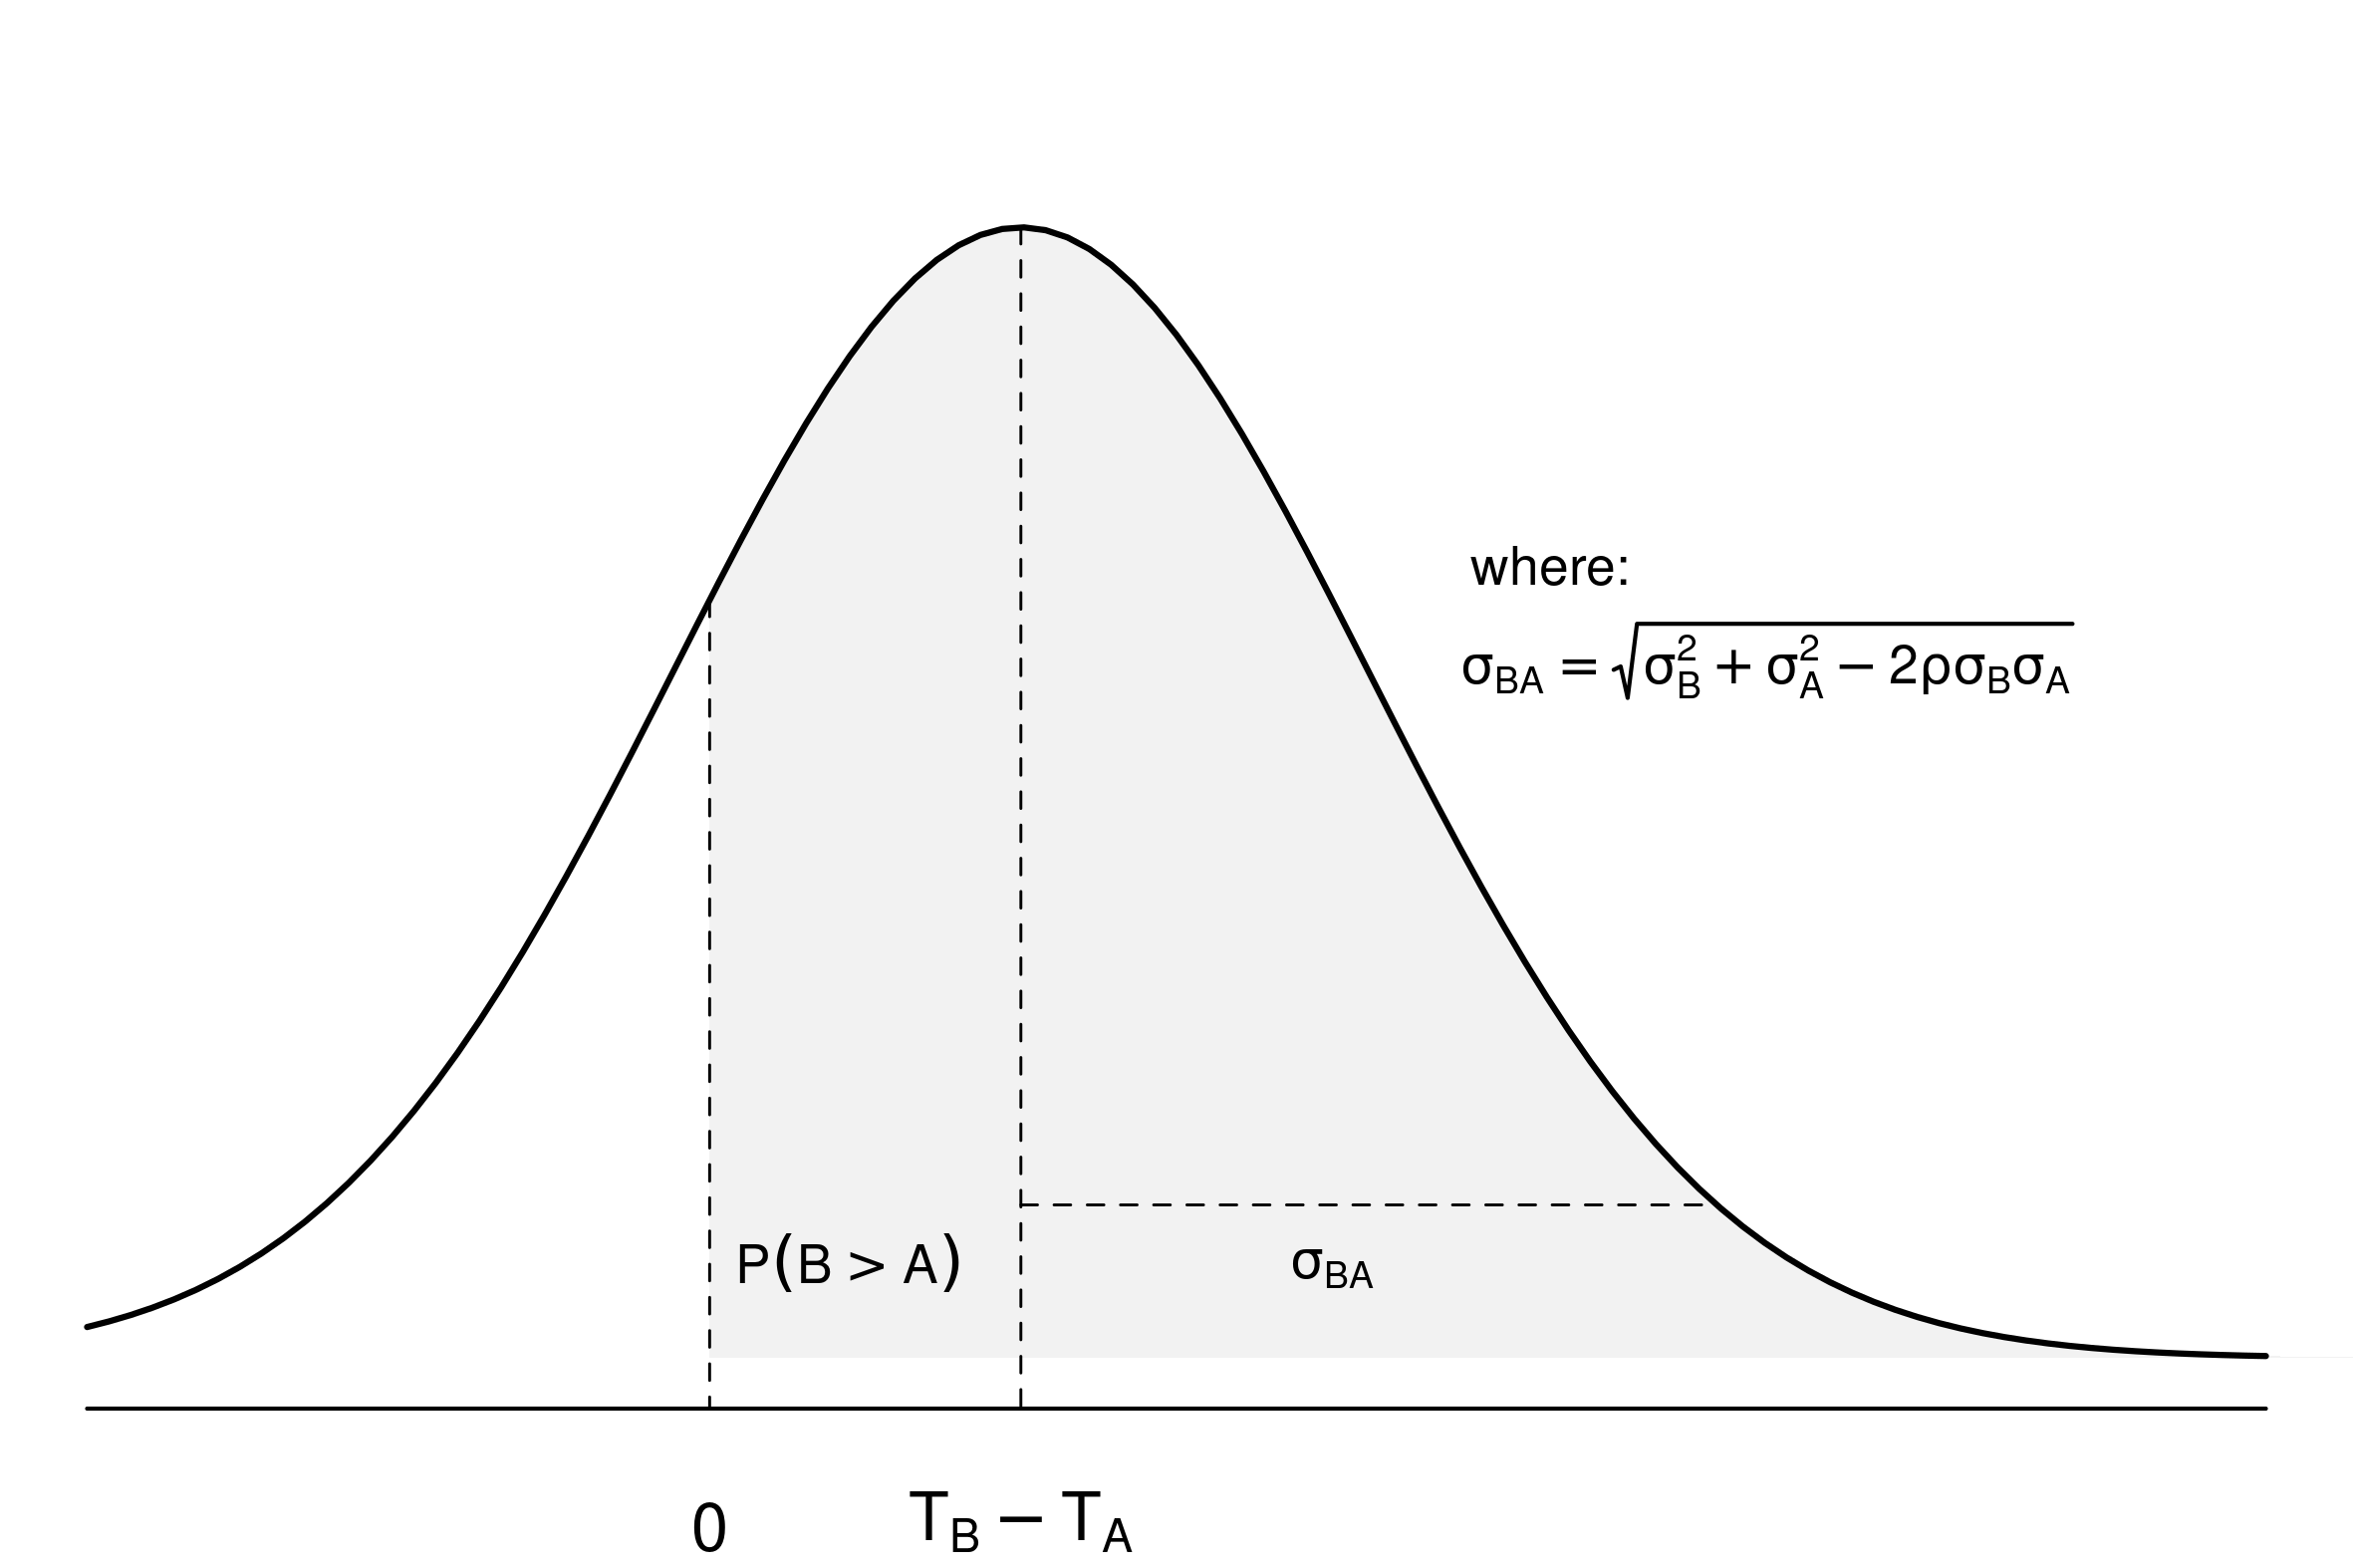
\includegraphics[width=1\linewidth,height=\textheight,keepaspectratio]{./images/png/discriminal_difference.png}

}

\subcaption{\label{fig-discriminal_difference}Discriminal difference}

\end{minipage}%

\caption{\label{fig-thurstone_theory}Hypothetical discriminal processes
and discriminant difference along a quality trait continuum for two
written texts.}

\end{figure}%

However, since the individual discriminal processes of the stimuli are
not directly observable, the theory introduces the \emph{law of
comparative judgment}. This law posits that in pairwise comparisons, a
judge perceives the stimulus with a discriminal process positioned
further along the trait continuum as possessing more of the trait
\citep{Bramley_2008}. This suggests that pairwise comparison outcomes
depend on the relative distance between stimuli, not their absolute
positions on the continuum. Indeed, the theory assumes that the
difference between the underlying discriminal processes of the stimuli,
referred to as the \emph{discriminal difference}, determines the
observed dichotomous outcome. Furthermore, the theory assumes that
because the individual discriminal processes form a Normal distribution
on the continuum, the discriminal difference will also conform to a
Normal distribution \citep{Andrich_1978}. In this distribution, the mode
(mean) represents the relative separation between the stimuli, and its
dispersion indicates the variability of that separation.

Figure~\ref{fig-discriminal_difference} illustrates the distribution of
the discriminal difference for the hypothetical texts depicted in
Figure~\ref{fig-discriminal_process}. The figure indicates that the
judge perceives Text B as having significantly higher quality than Text
A. Two key observations support this conclusion: the positive difference
between their modal discriminal processes \((T_{B} - T_{A} > 0)\) and
the probability area where the discriminal difference distinctly favors
Text B over Text A, represented by the shaded gray area denoted as
\(P(B > A)\). As a result, the dichotomous outcome of this comparison is
more likely to favor Text B over Text A.

\section{Two Prominent Issues in Traditional CJ
Practice}\label{sec-theory-issues}

Thurstone noted from the outset that his general form, described in
Section~\ref{sec-thurstone_theory}, led to a \emph{trait scaling
problem}. Specifically, the model required estimating more ``unknown''
parameters than the number of available pairwise comparisons
\citep[pp.~267]{Thurstone_1927b}. For instance, in a CJ experiment with
five texts, the general form would require estimating \(20\) parameters:
five modal discriminal processes, five discriminal dispersions, and
\(10\) correlations --one per comparison (see
Table~\ref{tbl-thurstone_cases}). However, a single judge could only
provide \({5 \choose 2} = 10\) unique comparisons, an insufficient data
set to estimate the required parameters.

To address this issue and facilitate the practical implementation of the
theory, Thurstone developed five cases derived from this general form,
each progressively incorporating additional simplifying assumptions. In
Case I, Thurstone postulated that pairs of stimuli would maintain a
constant correlation across all comparisons. In Case II, he allowed
multiple judges to undertake comparisons instead of confining
evaluations to a single judge. In Case III, he posited that there was no
correlation between stimuli. In Case IV, he assumed that the stimuli
exhibited similar dispersions. Finally, in Case V, he replaced this
assumption with the condition that stimuli had equal discriminal
dispersions. Table~\ref{tbl-thurstone_cases} summarizes the assumptions
of the general form and the five cases. For a detailed discussion of
these cases and their progression, refer to \citet{Thurstone_1927b} and
\citet[pp.~248--253]{Bramley_2008}.

\begin{table}

\caption{\label{tbl-thurstone_cases}Thurstones cases and their
asumptions}

\centering{

\includegraphics[width=1\linewidth,height=\textheight,keepaspectratio]{./images/png/thurstone_cases.png}

}

\end{table}%

However, Thurstone developed Case V prioritizing statistical simplicity
over precise trait measurement, and without providing clear guidance on
how to use its measurement scores for hypothesis testing. Specifically,
he cautioned that its use ``should not be made without (an) experimental
test'' \citep[pp.~270]{Thurstone_1927b}, as the case imposes the most
extensive set of simplifying assumptions
\citep{Bramley_2008, Kelly_et_al_2022} (see
Table~\ref{tbl-thurstone_cases}). Moreover, because Thurstone's primary
goal was to provide a ``rather coarse scaling'' of traits
\citep[pp.~269]{Thurstone_1927b} and ``allocate the compared stimuli on
this continuum'' \citep[pp.~269]{Thurstone_1927b}, he did not address
how to use the resulting measurement scores for hypothesis testing.
Thus, given these limitations, it is surprising that CJ research has
predominantly relied on Case V to measure different traits, raising
significant concerns about the reliability and validity of such
measurements in contexts where the case's assumptions may not hold
\citep{Kelly_et_al_2022, Andrich_1978}. Furthermore, although the CJ
practice has attempted to address the issue of hypothesis testing by
using the scores' point estimates or their transformations, a critical
question remains: Is this approach suitable for addressing these
inquiries?

Thus, this section discusses these two prominent issues. Specifically,
Section~\ref{sec-theory-issue1} examines the heavy reliance on
Thurstone's Case V assumptions in the statistical analysis of CJ data.
Conversely, Section~\ref{sec-theory-issue2} focuses on the apparent
disconnect between the approaches to trait measurement and hypothesis
testing in CJ.

\subsection{The Case V and the statistical analysis of CJ
data}\label{sec-theory-issue1}

As previously discussed, Case V remains the most widely used model in CJ
literature. This preference primarily stems from the BTL model, which
provides a simplified statistical representation of the case. The BTL
model mirrors the assumptions of Case V, with one notable distinction:
while Case V assumes a Normal distribution for the stimuli' discriminal
processes, the BTL model uses the more mathematically tractable Logistic
distribution \citep{Andrich_1978, Bramley_2008} (see
Table~\ref{tbl-thurstone_cases}). However, this substitution has minimal
impact on the model's estimation or interpretation because the
discriminal process scale is arbitrary up to a non-monotonic
transformation \citep{vanderLinden_et_al_2017_I, McElreath_2021}.
Furthermore, this limited impact is supported by the fact that the
Normal and Logistic distributions exhibit analogous statistical
properties, differing only by a scaling factor of approximately \(1.7\).

However, Thurstone acknowledged that some assumptions of Case V could be
problematic when researchers assess complex traits or heterogeneous
stimuli \citep{Thurstone_1927a}. Thus, given that modern CJ applications
often involve such traits and stimuli, two key assumptions of Case V,
and by extension, the BTL model, may not always hold in theory or
practice. These assumptions are the equal dispersion and zero
correlation between stimuli.

\subsubsection{The assumption of equal dispersions between
stimuli}\label{sec-theory-issue1a}

According to the theory, discrepancies in the discriminal dispersions of
stimuli shape the distribution of the discriminal difference, directly
influencing the outcome of pairwise comparisons. A thought experiment
can help illustrate this idea. In it, researchers observe the
discriminal processes for two texts, A and B, assuming that the
dispersion for Text A remains constant and that the two texts are
uncorrelated \((\rho=0)\). Figure~\ref{fig-dispersion} demonstrates that
an increase in the uncertainty associated with the perception of Text B
relative to Text A \((\sigma_{B} - \sigma_{A})\), broadens the
distribution of their discriminal difference. This broadening affects
the probability area where the discriminal difference distinctly favors
Text B over Text A, expressed as \(P(B>A)\), ultimately influencing the
comparison outcome. Additionally, the figure reveals that when the
discriminal dispersions of the texts are equal, as in the BTL model
\((\sigma_{B} - \sigma_{A}=0)\), the discriminal difference distribution
is more narrow than when the dispersions differ. As a result, the
discriminal difference is more likely to favor Text B over Text A, as it
is represented by the shaded gray area.

\begin{figure}

\begin{minipage}{0.50\linewidth}

\centering{

\includegraphics[width=1\linewidth,height=\textheight,keepaspectratio]{./images/png/dispersion.png}

}

\subcaption{\label{fig-dispersion}Discriminal Difference distribution
under varying discrepancies in stimuli dispersions}

\end{minipage}%
%
\begin{minipage}{0.50\linewidth}

\centering{

\includegraphics[width=1\linewidth,height=\textheight,keepaspectratio]{./images/png/correlation.png}

}

\subcaption{\label{fig-correlation}Discriminal Difference distribution
under varying levels of correlation between stimuli}

\end{minipage}%

\caption{\label{fig-casev_issues}The effect of dispersion discrepancies
and stimuli correlation on the distribution of the discriminal
difference.}

\end{figure}%

In experimental practice, however, the thought experiment occurs in
reverse. Researchers first observe the comparison outcome and then use
the BTL model to infer the discriminal difference between stimuli and
their respective discriminal processes \citep{Thurstone_1927a}.
Consequently, the outcome's ability to reflect \emph{true} differences
between stimuli largely depends on the validity of the model's
assumptions \citep{Kohler_et_al_2019}, in this case, the assumption of
equal dispersions. For instance, when the assumption accurately captures
the complexity of the data, the BTL model estimates a discriminal
difference distribution that accurately represents the \emph{true}
discriminal difference between the texts. This scenario is illustrated
in Figure~\ref{fig-dispersion}, when the model's discriminal difference
distribution aligns with the \emph{true} discriminal difference
distribution, represented by the thick continuous line corresponding to
\(\sigma_{B}-\sigma_{A}=0\). The accuracy of this discriminal difference
then ensures reliable estimates for the texts' discriminal processes.

Notably, while assuming equal dispersions simplifies the trait
measurement model, evidence from the CJ literature suggests that this
assumption may fail to capture the complexity of modern CJ data. In
particular, the assumption may not hold when researchers assess complex
traits or heterogeneous stimuli
\citep{Thurstone_1927a, Bramley_2008, Kelly_et_al_2022}, as these traits
and stimuli can introduce judgment discrepancies due to their unique
characteristics
\citep{vanDaal_et_al_2016, Lesterhuis_2018, Chambers_et_al_2022}.
Indeed, the CJ literature may already provide indications of such
discrepancies, particularly in the form of ``misfit'' statistics. For
instance, \emph{misfit texts} are those whose comparisons result in more
judgment discrepancies than those involving other texts
\citep{Pollitt_2004, Pollitt_2012b, Pollitt_2012a, Goossens_et_al_2018}.
These misfit texts may exhibit larger discriminal dispersions or
represent outliers --texts with distinctive characteristics that deviate
markedly from the rest of the sample \citep{Grubbs_1969}. In either
case, comparing misfit texts results in more judgment discrepancies, yet
the BTL model neither accounts for these cases nor offers any means to
address them.

Significant statistical and measurement issues can arise when the
assumption of equal dispersions between stimuli does not hold.
Specifically, the BTL model may overestimate the trait's reliability,
that is, the degree to which the outcome accurately reflects the
\emph{true} discriminal differences between stimuli. This
overestimation, in turn, results in spurious conclusions about these
differences \citep{McElreath_2020} and, by extension, about the
underlying discriminal processes of stimuli. Figure~\ref{fig-dispersion}
also illustrates this scenario when the model's discriminal difference
distribution aligns with the thick continuous line for
\(\sigma_{B}-\sigma_{A}=0\), while the \emph{true} discriminal
difference follows any discontinuous line where
\(\sigma_{B}-\sigma_{A} \neq 0\). Furthermore, if researchers
acknowledge that misfit statistics may represent outlying observations,
the common CJ practice of excluding stimuli based on these statistics
\citep{Pollitt_2012a, Pollitt_2012b, vanDaal_et_al_2016, Goossens_et_al_2018},
may unintentionally discard valuable information, introducing bias into
the trait estimates \citep[chap.~12]{Zimmerman_1994, McElreath_2020}.
The direction and magnitude of these biases remain unpredictable, as
they depend on which stimuli researchers exclude from the analysis.

\subsubsection{The assumption of zero correlation between
stimuli}\label{sec-theory-issue1b}

The correlation \(\rho\) measures how much the judges' perception of a
specific trait in one stimulus depends on their perception of the same
trait in another. As with the discriminal dispersions, this correlation
shapes the distribution of the discriminal difference, directly
impacting the outcomes of pairwise comparisons. A similar thought
experiment, as the one depicted in Section~\ref{sec-theory-issue1a}, can
illustrate this idea. The experiment only assumes that the discriminal
dispersions for both texts remain constant. Figure~\ref{fig-correlation}
reveals that as the correlation between the texts increases, the
distribution of their discriminal difference becomes narrower. This
narrowing affects the area under the curve where the discriminal
difference distinctly favors Text B over Text A, denoted as
\(P(B > A)\), thus influencing the comparison outcome. Furthermore, the
figure shows that when two texts are independent or uncorrelated
\((\rho=0)\), their discriminal difference is less narrow compared to
scenarios where the texts are positively correlated. As a result, the
discriminal difference is less likely to favor Text B over Text A, as it
is represented by the shaded gray area.

Thurstone assumed that stimuli were uncorrelated because judges' biases,
arising from two opposing and equally weighted effects occurring during
the pairwise comparisons, canceled each other out
\citep{Thurstone_1927b}. \citet{Andrich_1978} provided a mathematical
demonstration of this cancellation using the BTL model under the
assumption of discriminal processes with additive biases. However,
evidence from the CJ literature indicates that the assumption of zero
correlation does not hold in practice in at least two scenarios: when
intricate aspects of multidimensional, complex traits or heterogeneous
stimuli influence judges' perceptions or when additional hierarchical
structures are relevant to the stimuli.

In the first scenario, research on text quality suggests that when
judges evaluate multidimensional, complex traits or heterogeneous
stimuli, they often rely on various intricate characteristics of the
stimuli to form their judgments
\citep{vanDaal_et_al_2016, Lesterhuis_2018, Chambers_et_al_2022}. These
additional relevant characteristics, when assessed, are unlikely to be
equally weighted or opposing. As a result, they may exert an uneven
influence on judges' perceptions, creating biases that resist
cancellation. For example, this could occur when a judge assessing the
argumentative quality of a text places more weight on its grammatical
accuracy than other judges, thereby favoring texts with fewer errors but
weaker arguments. Furthermore, since the discriminal difference of the
stimuli becomes an observable outcome only through the judges'
perceptions, these biases could introduce dependencies between the
stimuli \citep{vanderLinden_et_al_2017_II}. While direct evidence for
this particular scenario is lacking, studies such as
\citet{Pollitt_et_al_2003} and \citet{vanDaal_et_al_2016} demonstrate
the presence of such biases, supporting the notion that the factors
influencing pairwise comparisons may not always cancel out.

In the second scenario, the shared context or inherent connections
introduced by additional hierarchical structures may create dependencies
between stimuli, a statistical phenomenon known as clustering
\citep{Everitt_et_al_2010}. For instance, when multiple texts are
produced by the same individual, these texts are likely to share common
features, such as writing style or even their general quality. Although
the CJ literature acknowledges the existence of such hierarchical
structures, the statistical approaches to account for this additional
source of dependence have been insufficient. For instance, when CJ data
incorporates multiple samples of stimuli from the same individuals,
researchers frequently rely on (averaged) point estimates of the BTL
scores to conduct subsequent analyses and tests at the individual level
\citep{Bramley_et_al_2019, Boonen_et_al_2020, Bouwer_et_al_2023, vanDaal_et_al_2017, Jones_et_al_2019, Gijsen_et_al_2021}.
However, this approach can introduce additional statistical and
measurement issues, which we discuss in greater detail in
Section~\ref{sec-theory-issue2}.

Thus, erroneously assuming zero correlation between stimuli can also
lead to significant statistical and measurement issues. Specifically,
neglecting judges' biases or relevant hierarchical structures can create
dimensional mismatches in the model, leading to the over- or
underestimation of trait reliability
\citep{Ackerman_1989, Hoyle_et_al_2023}. These inaccuracies can result
in spurious conclusions about the discriminal differences
\citep{McElreath_2020} and, by extension, the underlying discriminal
processes of the stimuli. This issue is illustrated in
Figure~\ref{fig-correlation} when the discriminal difference
distribution of the BTL scores follows the thick continuous line
\((\rho = 0)\), while the \emph{true} discriminal difference follows any
discontinuous line where \(\rho \neq 0\).

Finally, as discussed in the previous section, removing \emph{misfit}
judges based risks discarding valuable information and even introduce
bias into the trait estimates
\citep[chap.~12]{Zimmerman_1994, McElreath_2020}. The direction and
magnitude of these biases remain unpredictable because they depend on
which judges researchers exclude from the analysis. \emph{Misfit judges}
are those whose evaluations deviate substantially from the shared
consensus due to the unique characteristics of either the stimuli or the
judges themselves
\citep{Pollitt_2012a, Pollitt_2012b, vanDaal_et_al_2016, Goossens_et_al_2018}.

\subsection{The disconnect between trait measurement and hypothesis
testing}\label{sec-theory-issue2}

Building on the previous section, it is clear that, researchers
typically rely on the BTL model to measure a trait and place the
compared stimuli along its continuum \citep{Thurstone_1927b}.
Additionally, the CJ literature shows that researchers frequently use
point estimates of BTL scores or their transformations to conduct
further analyses or hypothesis tests. For example, researchers have used
these scores to identify `misfit' judges and stimuli
\citep{Pollitt_2012b, vanDaal_et_al_2016, Goossens_et_al_2018}, detect
biases in judges' ratings \citep{Pollitt_et_al_2003, Pollitt_2012b},
calculate correlations with other assessment methods
\citep{Goossens_et_al_2018, Bouwer_et_al_2023}, or test hypotheses
related to the underlying trait of interest
\citep{Casalicchio_et_al_2015, Bramley_et_al_2019, Boonen_et_al_2020, Bouwer_et_al_2023, vanDaal_et_al_2017, Jones_et_al_2019, Gijsen_et_al_2021}.

Nevertheless, while separating the trait measurement and hypothesis
testing processes simplifies the analysis of CJ data, the statistical
literature cautions against relying solely on the point estimates of BTL
scores to conduct further analyses or hypothesis tests, as this practice
can undermine the resulting statistical conclusions. A key consideration
is that BTL scores are parameter estimates that inherently carry
uncertainty (measurement error). Ignoring this uncertainty can bias the
analysis and reduce the precision of hypothesis tests. The direction and
magnitude of such biases are often unpredictable. Results may be
attenuated, exaggerated, or remain unaffected depending on the degree of
uncertainty in the scores and the actual effects being tested
\citep{McElreath_2020, Kline_et_al_2023, Hoyle_et_al_2023}. Furthermore,
the reduced precision in hypothesis tests diminishes their statistical
power, increasing the likelihood of committing type-I or type-II errors
\citep{McElreath_2020}. Figure~\ref{fig-measurement_error} illustrates
these issues, demonstrating how neglecting measurement error
\((\sigma_{T})\) by relying only on outcome averages can reduce the
precision of a predictor's estimated effect.

\begin{figure}

\centering{

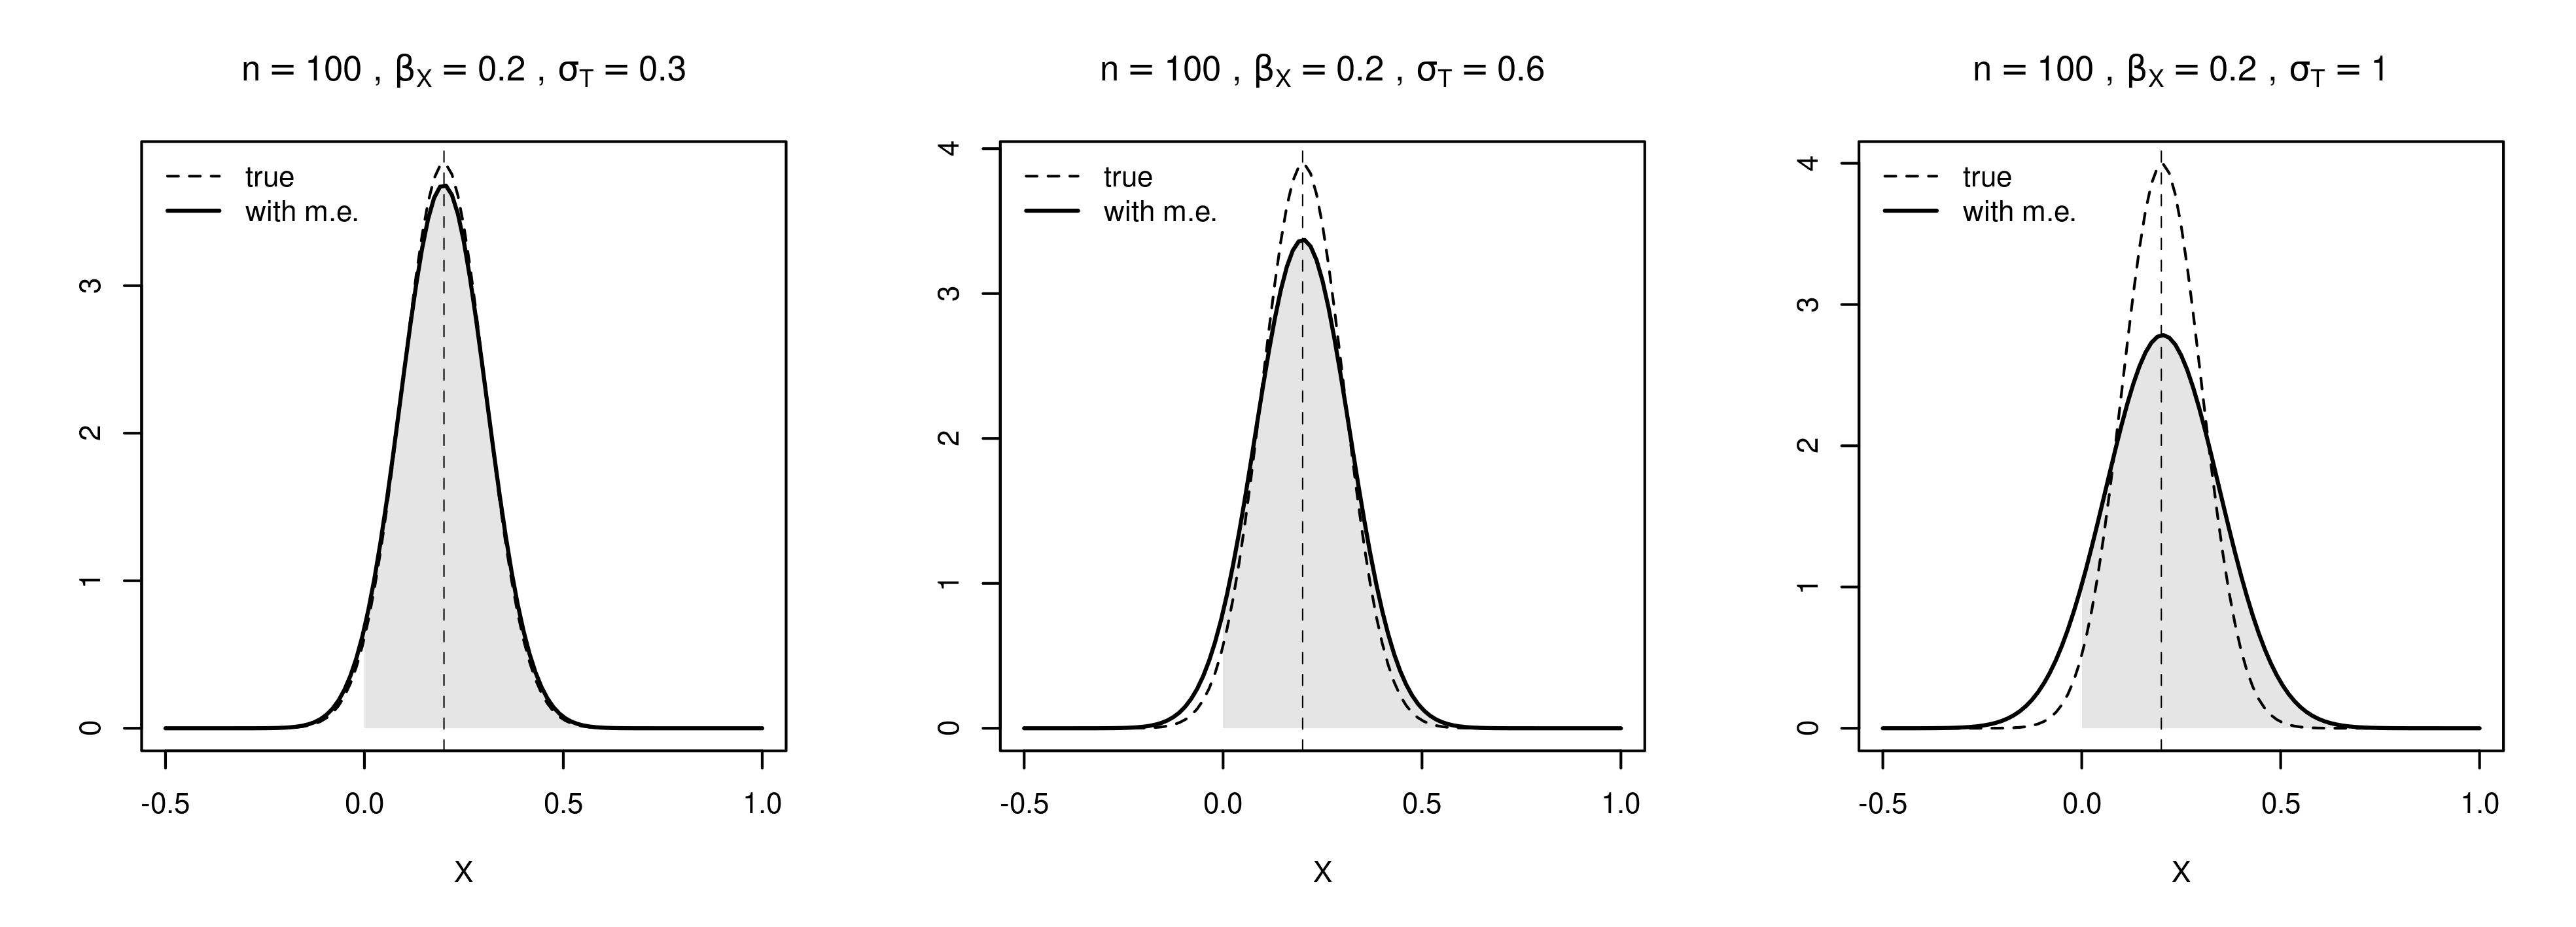
\includegraphics[width=1\linewidth,height=\textheight,keepaspectratio]{./images/png/measurement_error.png}

}

\caption{\label{fig-measurement_error}The effect of outcome uncertainty
\(\sigma_{T}\) on the estimation of an effect \(\beta_{X}\) linked to
the predictor. The example assumes a sample size \(n=100\) and an
uncertainty that increases from left to right.}

\end{figure}%

In aggregate, the heavy reliance on Thurstone's Case V assumptions in
the statistical analysis of comparative data can compromise the
reliability of trait estimates. This overreliance may also undermine
their validity \citep{Perron_et_al_2015}, particularly when coupled with
the disconnect between the trait measurement and hypothesis testing
processes. However, the structural approach to causal inference can
address these issues by offering a systematic and integrated framework
that strengthens measurement reliability and validity while enhancing
the statistical accuracy of hypothesis tests.

\section{Extending Thurstone's general form}\label{sec-theoretical}

The \emph{structural approach} to causal inference provides a formal
framework for identifying causes and estimating their effects using
data. The approach uses structural causal models (SCMs) and directed
acyclic graphs (DAGs)
\citep{Pearl_2009, Pearl_et_al_2016, Gross_et_al_2018, Neal_2020} to
formally and graphically represent the assumed causal structure of a
system, such as the one found in CJ experiments. Essentially, SCMs and
DAGs function as \emph{conceptual models} on which identification
analysis rests. \emph{Identification analysis} helps researchers to
determine whether an estimator can accurately compute an estimand based
solely on its (causal) assumptions, regardless of random variability
\citep{Schuessler_et_al_2023}. Here, \emph{estimands} represent the
specific quantities researchers aim to determine
\citep{Everitt_et_al_2010}. \emph{Estimators} denote the methods or
functions that transform data into an estimate, while \emph{estimates}
are the numerical values approximating the estimand
\citep{Neal_2020, Everitt_et_al_2010}.

A motivating example that will appear in the rest of the document
clarifies these concepts. In this example, researchers aim to determine:
``To what extent do different teaching methods influence students'
ability to produce high-quality written texts?'' To investigate this, a
researcher designs a CJ experiment by randomly assigning students
(individuals) to two groups, each receiving a different teaching method.
Judges then compare pairs of students' written texts (stimuli) to
produce a dichotomous outcome reflecting the relative quality of each
text (trait). Based on this setup, researchers can reformulate the
research question as the estimand: ``\emph{On average}, is there a
difference in the ability to produce high-quality written texts between
the two groups of students?''. Following current CJ practices,
researchers rely on estimates from the BTL model, or its
transformations, to approximate this estimand.

However, Section~\ref{sec-theory-issues} presents compelling evidence
that Thurstone's Case V, and by extension the BTL model, suffers from
several statistical and measurement limitations. These limitations
hinder the model's ability to identify various estimands relevant to CJ
inquiries, including the one described in the example. Identification is
crucial because it is a necessary condition for ensuring consistent
estimators. \emph{Consistency} refers to the property of an estimator
whose estimates converge to the ``true'' value of the estimand as the
data size approaches infinity \citep{Everitt_et_al_2010}. Without
identification, consistency cannot be achieved, even with ``infinite''
and error-free data. Thus, deriving meaningful insights from finite data
becomes impossible \citep{Schuessler_et_al_2023}.

Fortunately, SCMs and DAGs support identification analysis through two
key advantages\footnote{These topics are beyond the scope of this study,
  thus, readers seeking a more profound understanding can refer to
  introductory papers such as \citet{Pearl_2010}, \citet{Rohrer_2018},
  \citet{Pearl_2019}, and \citet{Cinelli_et_al_2020}, and introductory
  books like \citet{Pearl_et_al_2018}, \citet{Neal_2020}, and
  \citet{McElreath_2020} are useful. For more advanced study, seminal
  papers such as \citet{Neyman_et_al_1923}, \citet{Rubin_1974},
  \citet{Spirtes_et_al_1991}, and \citet{Sekhon_2009}, along with books
  such as \citet{Pearl_2009}, \citet{Morgan_et_al_2014}, and
  \citet{Hernan_et_al_2020}, are recommended.}. First, regardless of
complexity, they can represent various causal structures using only five
fundamental building blocks \citep{Neal_2020, McElreath_2024}. This
feature allows researchers to decompose complex structures into
manageable components, facilitating their analysis. Second, they depict
causal relationships in a non-parametric way. This flexibility enables
feasible identification strategies without requiring specification of
the types of variables, the functional forms relating them, or the
parameters of those functional forms \citep{Pearl_et_al_2016}.

Thus, this section addresses the issues identified in
Section~\ref{sec-theory-issues} by extending Thurstone's general form
using the structural approach to Causal inference. Specifically, it
combines the core theoretical principles outlined in
Section~\ref{sec-thurstone_theory} with key assessment design features
relevant to CJ experiments, such as the selection of judges, stimuli,
and comparisons. In addition to improving statistical accuracy and
strengthening measurement reliability and validity, the approach offers
two key advantages. First, it clarifies the interactions among all
actors and processes involved in CJ experiments. Second, it shifts the
current comparative data analysis paradigm from passively accepting the
model assumptions to actively testing whether those assumptions fit the
data under analysis.

Accordingly, Section~\ref{sec-theory-theoretical_P} incorporates the
theoretical principles into what we refer to as the
\emph{conceptual-population model}. This model assumes an idealized
scenario where researchers have access to a \emph{conceptual population}
of comparative data, that is, data representing all repeated judgments
made by every available judge for each pair of stimuli produced by each
pair of individuals in the population. Conversely,
Section~\ref{sec-theory-theoretical_SC} integrates the assessment design
features into what we refer to as the \emph{sample-comparison model}.
This model assumes a more realistic scenario where researchers only have
access to a sample of judges, individuals, stimuli, and comparisons from
the conceptual population.

\subsection{The conceptual-population
model}\label{sec-theory-theoretical_P}

In the conceptual-population model, the idealized scenario of a
\emph{conceptual population} of comparative data enables the integration
of Thurstone's theoretical principles and provides a foundation for
proposing innovations aimed at addressing some of the issues discussed
in Section~\ref{sec-theory-issues}.

\subsubsection{Integrating the first theoretical
principles}\label{sec-theory-theoretical_P1}

Before incorporating the first theoretical principles of Thurstone's
theory, it is essential to further define SCMs. SCMs are formal
mathematical models characterized by a set of \emph{endogenous}
variables \(V\), a set of \emph{exogenous} variables \(E\), and a set of
functions \(F\) \citep{Pearl_2009, Cinelli_et_al_2020}. Endogenous
variables are those whose causal mechanisms a researcher chooses to
model \citep{Neal_2020}. In contrast, exogenous variables represent
\emph{errors} or \emph{disturbances} arising from omitted factors that
the investigator chooses not to model explicitly \citep{Pearl_2009}.
Lastly, the functions, referred to as \emph{structural equations},
express the endogenous variables as non-parametric functions of other
endogenous and exogenous variables. These functions use the symbol
`\(:=\)' to denote the asymmetrical causal dependence between variables
and the symbol `\(\:\bot\:\)' to represent \emph{d-separation}, a
concept akin to (conditional) independence.

SCM~\ref{fig-cj03_scm} presents the first theoretical principles
embedded in the conceptual-population model, which evaluates the impact
of different teaching methods on students' writing ability. This SCM
outlines the relationship between the conceptual-population outcome
\((O^{cp}_{iahbjk})\) and several related variables. The subscripts
\(i\) and \(h\) identify the students who authored the texts (i.e., the
individuals). The indices \(a\) and \(b\) represent the texts under
comparison (i.e., the stimuli). The index \(j\) indicates the judge
conducting the comparison, while the index \(k\) captures \emph{repeated
measures designs} \citep[pp.~366-376]{Lawson_2015}, accounting for
experimental conditions where a judge compares the same pair of stimuli
multiple times. Thus, the indexing system supports comparisons between
different texts written by the same student \((i = h;\) \(a \neq b)\)
and between texts written by distinct students \((i \neq h;\) where
\(a = b\) is permitted\()\), each judged once or repeatedly by all
judges \((j = 1,\dots,n_{J};\) \(k = 1,\dots,n_K;\) where \(n_{J}>1\)
and \(n_{K}\geq1)\). However, it excludes cases where a judge compares a
student's text to itself, whether once or multiple times \((i = h;\)
\(a = b;\) \(j = 1,\dots,n_{J};\) \(k = 1,\dots,n_{K};\) where
\(n_{J}>1\) and \(n_{K}\geq1)\), as such comparison lacks practical
relevance within the CJ framework. Here, \(n_{J}\) indicates the total
number of judges, and \(n_{K}\) denotes the number of repeated judgments
each judge performs.

In line with Thurstone's theory, SCM~\ref{fig-cj03_scm} depicts the
texts' discriminal processes \((T_{ia}, T_{hb})\) and their discriminal
difference \((D_{iahbjk})\) (see Section~\ref{sec-thurstone_theory}).
Additionally, based on the arguments developed in
Section~\ref{sec-theory-issue1b}, the SCM incorporates the judges'
biases \((B_{kj})\). Together with the outcome, these variables
constitute the preliminary set of endogenous variables,
\(V = \{ O_{iahbjk}, D_{iahbjk}, T_{ia}, T_{hb}, B_{kj} \}\). Finally,
the SCM presents the preliminary set of structural equations,
\(F = \{ f_{O}, f_{D} \}\), which define the non-parametric dependencies
among these variables.

\begin{figure}[H]

\begin{minipage}{\linewidth}

\centering{

\[
\begin{aligned}
  O^{cp}_{iahbjk} & := f_{O}(D_{iahbjk}) \\
  D_{iahbjk} & := f_{D}(T_{ia}, T_{hb}, B_{jk})
\end{aligned}
\]

}

\subcaption{\label{fig-cj03_scm}SCM}

\end{minipage}%
\newline
\begin{minipage}{\linewidth}

\centering{

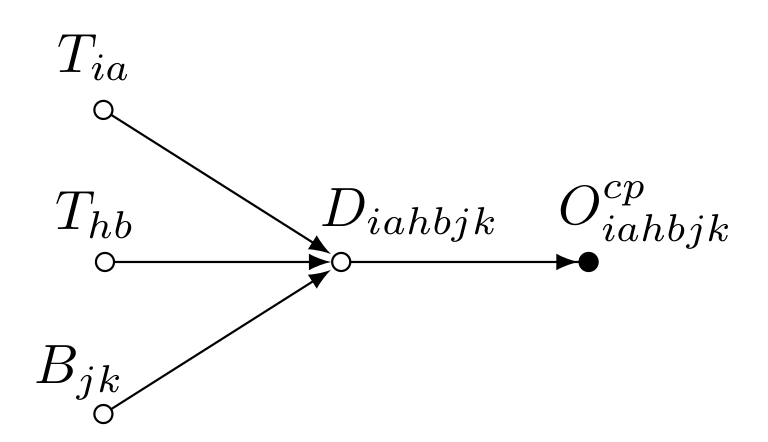
\includegraphics[width=0.35\linewidth,height=\textheight,keepaspectratio]{./images/png/CJ_TM_03.png}

}

\subcaption{\label{fig-cj03_dag}DAG}

\end{minipage}%

\caption{\label{fig-cj03}Conceptual-population model, scalar form.}

\end{figure}%

Notably, every SCM has an associated DAG
\citep{Pearl_et_al_2016, Cinelli_et_al_2020}. A DAG is a \emph{graph}
consisting of nodes connected by edges, where nodes represent random
variables. The term \emph{directed} indicates that edges or arrows
extend from one node to another, indicating the direction of causal
influence. The absence of an edge implies no direct relationship between
the nodes. The term \emph{acyclic} means that the causal influences do
not form loops, ensuring the influences do not cycle back on themselves
\citep{McElreath_2020}. DAGs conventionally depict observed variables as
solid black circles and unobserved (latent) variables as open circles
\citep{Morgan_et_al_2014}. Although DAGs conventionally omit exogenous
variables for simplicity, the DAGs presented in this section includes
exogenous variables to improve clarity and reveal potential issues
related to conditioning and confounding \citep{Cinelli_et_al_2020}.

Figure~\ref{fig-cj03_dag} displays the DAG corresponding to
SCM~\ref{fig-cj03_scm}, illustrating the expected causal relationships
outlined in Thurstone's theory. The graph shows that the discriminal
processes of the texts \((T_{ia}, T_{hb})\) influence their discriminal
difference \((D_{iahbjk})\), which in turn determines the outcome
\((O^{cp}_{iahbjk})\). It also highlights the influence of judges'
biases \((B_{kj})\) on the discriminal difference. Additionally, the DAG
differentiates between observed endogenous variables, such as the
outcome (solid black circle), and latent endogenous variables, including
the texts' discriminal processes, their discriminal difference, and the
judges' biases (open circles).

\subsubsection{\texorpdfstring{The \emph{conceptual population} data
structure}{The conceptual population data structure}}\label{sec-theory-theoretical_P2}

Although specifying a data structure is not mandatory when using SCMs
and DAGs, defining one in this case can improve clarity and facilitate
the description of the system. Thus, to re-express the scalar form of
the CJ system shown in Figure~\ref{fig-cj03} into an equivalent
vectorized form, we first define the vectors \(I\) and \(J\), along with
the matrices \(IA\) and \(JK\), as follows:
\begin{equation}\phantomsection\label{eq-mat11}{
I = \begin{bmatrix}
1 \\
\vdots \\
i \\
\vdots \\
h \\
\vdots \\
n_{I}
\end{bmatrix} ; \;
J = \begin{bmatrix}
1 \\
\vdots \\
j \\
\vdots \\
n_{J}
\end{bmatrix} ; \;
IA = \begin{bmatrix}
1 & 1 \\
\vdots & \vdots \\
1 & n_{A} \\
\vdots & \vdots \\
i & a \\
\vdots & \vdots \\
h & b \\
\vdots & \vdots \\
n_{I} & 1 \\
\vdots & \vdots \\
n_{I} & n_{A}
\end{bmatrix} ; \;
JK = \begin{bmatrix}
1 & 1 \\
\vdots & \vdots \\
1 & n_{K} \\
\vdots & \vdots \\
j & k \\
\vdots & \vdots \\
n_{J} & 1 \\
\vdots & \vdots \\
n_{J} & n_{K}
\end{bmatrix}
}\end{equation}

Here, each element of \(I\) represents a unique individual \(i\) or
\(h\), where \(n_{I}\) denotes the total number of individuals.
Similarly, each element of \(J\) corresponds to a unique judge \(j\),
with \(n_{J}\) indicating the total number of judges. Moreover, each row
of \(IA\) represents a unique pairing of individuals \(i, h\) with
stimuli \(a, b\). As a result, the matrix \(IA\) contains
\(n_{I} \cdot n_{A}\) rows and \(2\) columns, where \(n_{A}\) specifies
the number of stimuli available per individual. Likewise, each row of
\(JK\) associates a judge \(j\) with a (repeated) judgment index \(k\).
Consequently, the matrix \(JK\) has \(n_{J} \cdot n_{K}\) rows and \(2\)
columns, where \(n_{K}\) indicates the number of repeated judgments each
judge makes.

Additionally, we construct the matrix \(R\) to map each row of the
\(IA\) matrix with a corresponding row from the \(JK\) matrix. Thus,
this matrix has \(n\) rows and \(6\) columns, where
\(n = {n_{I} \cdot n_{A} \choose 2} \cdot n_{J} \cdot n_{K}\). Here, the
term \({n_{I} \cdot n_{A} \choose 2}\) represents the binomial
coefficient, which quantifies the total number of unique comparisons
possible between every pair of stimuli generated by each pair of
individuals in the population. Thus, we define the matrix as follows:

\begin{equation}\phantomsection\label{eq-mat12}{
R = \begin{bmatrix}
1 & 1 & 1 & 2 & 1 & 1 \\
\vdots & \vdots & \vdots & \vdots & \vdots & \vdots\\
1 & 1 & 1 & 2 & 1 & n_{K} \\
\vdots & \vdots & \vdots & \vdots & \vdots & \vdots\\
i & a & h & b & j & k \\
\vdots & \vdots & \vdots & \vdots & \vdots & \vdots\\
n_{I} & n_{A}-1 & n_{I} & n_{A} & n_{J} & 1 \\
\vdots & \vdots & \vdots & \vdots & \vdots & \vdots\\
n_{I} & n_{A}-1 & n_{I} & n_{A} & n_{J} & n_{K}
\end{bmatrix}
}\end{equation}

It is easier to visualize the structure of these vectors and matrices by
considering an example where \(n_{I} = 5\), \(n_{A} = 2\),
\(n_{J} = 3\), and \(n_{K} = 3\). In this simple case, the vectors and
matrices described in equations (\ref{eq-mat11}) and (\ref{eq-mat12})
take the following form:
\begin{equation}\phantomsection\label{eq-mat13}{
I = \begin{bmatrix}
1 \\
2 \\
3 \\
4 \\
5 
\end{bmatrix} ; \;
J = \begin{bmatrix}
1 \\
2 \\
3 
\end{bmatrix} ; \;
IA = \begin{bmatrix}
1 & 1 \\
1 & 2 \\
2 & 1 \\
2 & 2 \\
3 & 1 \\
3 & 2 \\
4 & 1 \\
4 & 2 \\
5 & 1 \\
5 & 2 
\end{bmatrix} ; \;
JK = \begin{bmatrix}
1 & 1 \\
1 & 2 \\
1 & 3 \\
2 & 1 \\
2 & 2 \\
2 & 3 \\
3 & 1 \\
3 & 2 \\
3 & 3 
\end{bmatrix} ; \;
R = \begin{bmatrix}
1 & 1 & 1 & 2 & 1 & 1 \\
1 & 1 & 1 & 2 & 1 & 2 \\
1 & 1 & 1 & 2 & 1 & 3 \\
\vdots & \vdots & \vdots & \vdots & \vdots & \vdots\\
1 & 1 & 5 & 2 & 1 & 1 \\
1 & 1 & 5 & 2 & 1 & 2 \\
1 & 1 & 5 & 2 & 1 & 3 \\
\vdots & \vdots & \vdots & \vdots & \vdots & \vdots\\
4 & 2 & 5 & 2 & 3 & 1 \\
4 & 2 & 5 & 2 & 3 & 2 \\
4 & 2 & 5 & 2 & 3 & 3 \\
5 & 1 & 5 & 2 & 3 & 1 \\
5 & 1 & 5 & 2 & 3 & 2 \\
5 & 1 & 5 & 2 & 3 & 3 
\end{bmatrix}
}\end{equation}

Now, using equations (\ref{eq-mat11}) and (\ref{eq-mat12}), we can
re-express SCM~\ref{fig-cj03_scm} and DAG~\ref{fig-cj03_dag} in an
equivalent vectorized form, as shown in Figure~\ref{fig-cj04}. In this
depiction, the outcome \(O^{cp}_{R}\), the texts' discriminal difference
\(D_{R}\), their discriminal processes \(T_{IA}\), and the judges'
biases \(B_{JK}\) are represented as vectors rather than scalar values.
These vectors capture all the observations from the conceptual
population. Specifically, \(O^{cp}_{R}\) and \(D_{R}\) are observed and
latent vectors of length \(n\), respectively. Moreover, \(T_{IA}\) and
\(B_{JK}\) are latent vectors of lengths \(n_{I} \cdot n_{A}\) and
\(n_{J} \cdot n_{K}\), respectively.

\begin{figure}[H]

\begin{minipage}{\linewidth}

\centering{

\[
\begin{aligned}
  O^{cp}_{R} & := f_{O}(D_{R}) \\
  D_{R} & := f_{D}(T_{IA}, B_{JK})
\end{aligned}
\]

}

\subcaption{\label{fig-cj04_scm}SCM}

\end{minipage}%
\newline
\begin{minipage}{\linewidth}

\centering{

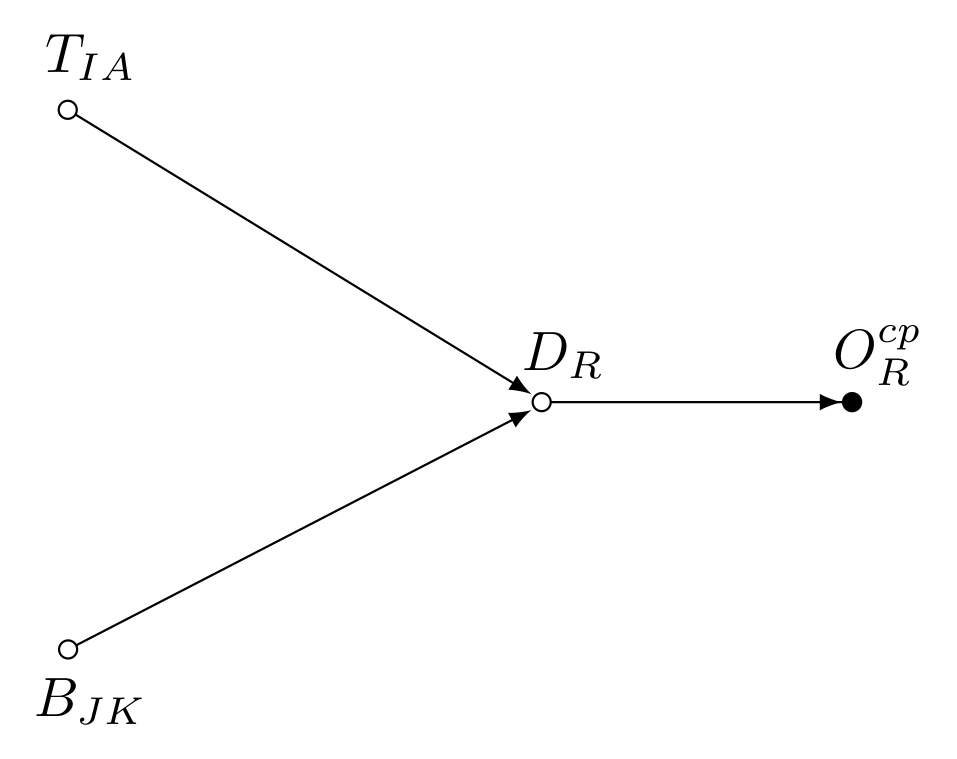
\includegraphics[width=0.44\linewidth,height=\textheight,keepaspectratio]{./images/png/CJ_TM_04.png}

}

\subcaption{\label{fig-cj04_dag}DAG}

\end{minipage}%

\caption{\label{fig-cj04}Conceptual-population model, initial vectorized
form.}

\end{figure}%

\subsubsection{Integrating hierarchical structural
components}\label{sec-theory-theoretical_P3}

Building on the principles of Structural Equation Modeling (SEM)
\citep{Hoyle_et_al_2023} and Item Response Theory (IRT)
\citep{Fox_2010, vanderLinden_et_al_2017_I}, the conceptual-population
model integrates two \emph{hierarchical structural components} to
examine how different teaching methods influence students' writing
ability. Each structural component defines how observed or latent
variables affect the primary latent variable of interest
\citep{Everitt_et_al_2010}. Their hierarchical nature enables
researchers to test hypotheses considering the hierarchical structure of
stimuli (see Section~\ref{sec-theory-issue1b}) and the uncertainties in
trait estimation (see Section~\ref{sec-theory-issue2}).

The top branch of DAG~\ref{fig-cj09_dag} illustrates the first
component, where \emph{relevant} \footnote{\emph{Relevant variables} are
  those that satisfy the \emph{backdoor criterion} \citep[pp
  37]{Neal_2020}, that is, they belong to a \emph{sufficient adjustment
  set} \citep{Pearl_2009, Pearl_et_al_2016, Morgan_et_al_2014}. A
  \emph{sufficient} set (potentially empty) blocks all non-causal paths
  between a predictor and an outcome without opening new ones
  \citep{Pearl_2009}. Refer also to footnote 1.} student-related
variables \((X_{I})\), such as teaching method, and students'
idiosyncratic errors \(e_{I}\) causally influence the latent variable
representing students' writing-quality trait \((T_{I})\). The error term
\(e_{I}\) captures variations in students' traits unexplained by
\(X_{I}\). Here, \(X_{I}\) is an observed matrix with \(n_{I}\) rows and
\(q_{I}\) columns (variables), and both \(e_{I}\) and \(T_{I}\) are
latent vectors of length \(n_{I}\). Additionally, this branch shows how
\(T_{I}\), along with \emph{relevant} \footnote{refer to footnote 2.}
text-related variables \((X_{IA})\) (e.g., text length), and texts'
idiosyncratic errors \(e_{IA}\) causally influence the texts'
written-quality trait \((T_{IA})\), the first primary latent variable of
interest. The error term \(e_{IA}\) captures variations in the texts'
traits that remain unexplained by \(T_{I}\) or \(X_{IA}\). Here,
\(X_{IA}\) is an observed matrix with dimensions \(n_{I} \cdot n_{A}\)
rows and \(q_{IA}\) columns (variables), while \(e_{IA}\) and \(T_{IA}\)
are latent matrices with \(n_{I}\) rows and \(n_{A}\) columns.

Similarly, the bottom branch of DAG~\ref{fig-cj09_dag} depicts the
second component, where \emph{relevant} \footnote{refer to footnote 2.}
judge-related variables \((Z_{J})\), such as judgment expertise, and
judges' idiosyncratic errors \(e_{J}\) causally influence the latent
variable representing judges' bias \((B_{J})\). The error \(e_{J}\)
captures variations in judges' bias unexplained by \(Z_{J}\). Here,
\(Z_{J}\) is an observed matrix with \(n_{J}\) rows and \(q_{J}\)
columns (variables), and both \(e_{J}\) and \(B_{J}\) are latent vectors
of length \(n_{J}\). Furthermore, the branch shows how \(B_{J}\), along
with \emph{relevant} \footnote{refer to footnote 2.} judgment-related
variables \((Z_{JK})\) (e.g., the number of judgments a judge makes),
and judgments' idiosyncratic errors \(e_{JK}\) causally influence the
judges' biases associated with each text \(B_{JK}\), the second primary
latent variable of interest. The error \(e_{JK}\) captures variations in
judgments unexplained by \(B_{J}\) or \(Z_{JK}\). Here, \(Z_{JK}\) is an
observed matrix with dimension \(n_{J} \cdot n_{K}\) rows and \(q_{JK}\)
columns (variables), while \(e_{JK}\) and \(B_{JK}\) are latent latent
matrices with \(n_{J}\) rows and \(n_{K}\) columns

Notably, all variables and functions shown in SCM~\ref{fig-cj09_scm} and
DAG~\ref{fig-cj09_dag} are part of the set of endogenous variables
\(V\), structural equations \(F\), and exogenous variables \(E\) for the
conceptual-population model. Additionally, the figures demonstrate that
all exogenous variables are independent of one another, as indicated by
the relationships \(e_{IA} \:\bot\:\{ e_{I}, e_{JK}, e_{J} \}\),
\(e_{I} \:\bot\:\{ e_{JK}, e_{J} \}\) and \(e_{JK} \:\bot\:e_{J}\).

Overall, the conceptual-population model extends Thurstone's general
form by introducing key innovations to address the limitations discussed
in Section~\ref{sec-theory-issue1b} and Section~\ref{sec-theory-issue2}.
These enhancements include accounting for judges' biases and integrating
hierarchical structural components. Nevertheless, despite its promise of
enhancing measurement accuracy and precision, the model still depends on
the unrealistic assumption that researchers have access to a
\emph{conceptual population}. Since researchers rarely meet this
assumption in practice, they must consider a more realistic scenario.

\begin{figure}[H]

\begin{minipage}{\linewidth}

\centering{

\[
\begin{aligned}
  O^{cp}_{R} & := f_{O}(D_{R}) \\
  D_{R} & := f_{D}(T_{IA}, B_{JK}) \\
  T_{IA} & := f_{T}(T_{I}, X_{IA}, e_{IA}) \\
  T_{I} & := f_{T}(X_{I}, e_{I}) \\
  B_{JK} & := f_{B}(B_{J}, Z_{JK}, e_{JK}) \\
  B_{J} & := f_{B}(Z_{J}, e_{J}) \\
  e_{I} & \:\bot\:\{ e_{J}, e_{IA}, e_{JK} \} \\
  e_{J} & \:\bot\:\{ e_{IA}, e_{JK} \} \\
  e_{IA} & \:\bot\:e_{JK} 
\end{aligned}
\]

}

\subcaption{\label{fig-cj09_scm}SCM}

\end{minipage}%
\newline
\begin{minipage}{\linewidth}

\centering{

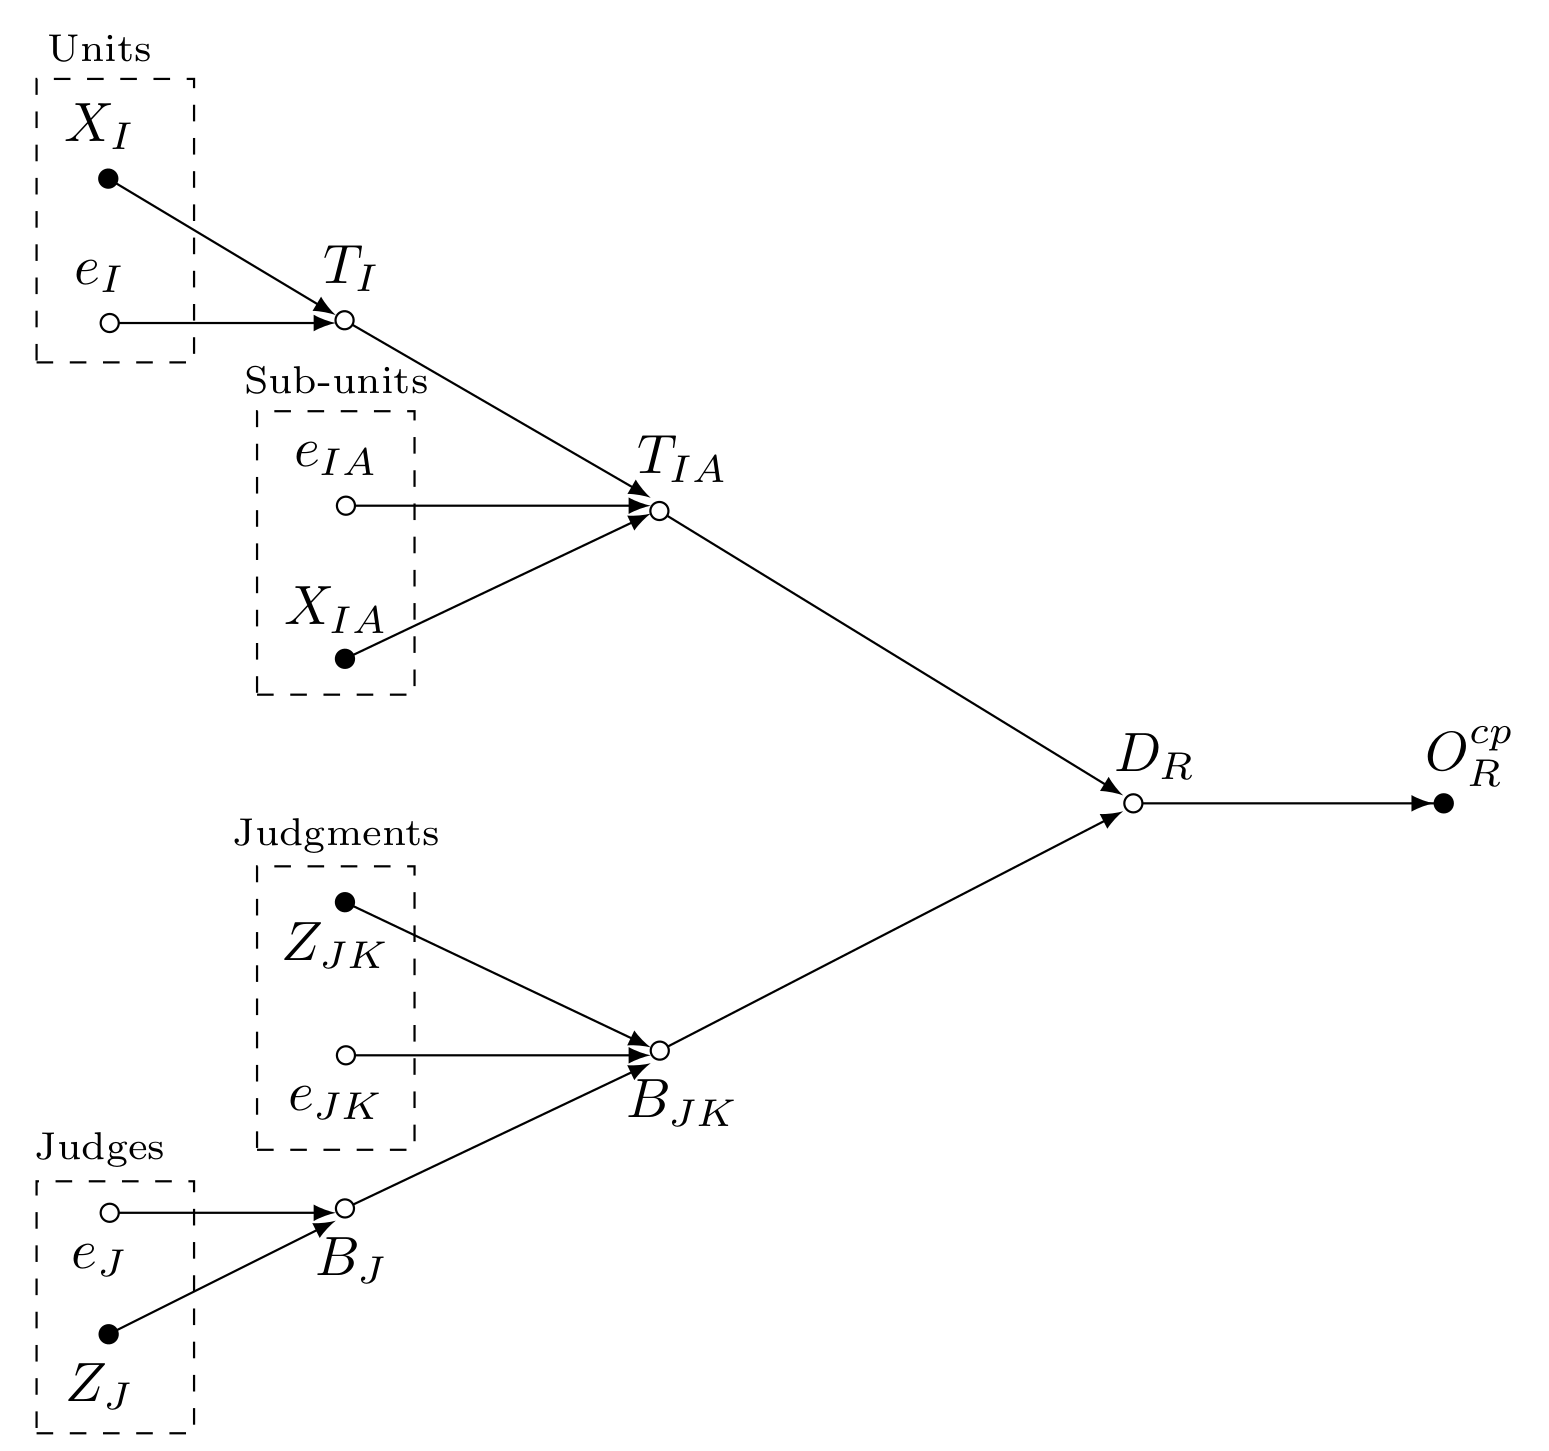
\includegraphics[width=0.7\linewidth,height=\textheight,keepaspectratio]{./images/png/CJ_TM_09.png}

}

\subcaption{\label{fig-cj09_dag}DAG}

\end{minipage}%

\caption{\label{fig-cj09}Conceptual-population model, final vectorized
form.}

\end{figure}%

\subsection{The sample-comparison
model}\label{sec-theory-theoretical_SC}

The sample-comparison model presents a more realistic scenario than the
conceptual-population model. In
Section~\ref{sec-theory-theoretical_SC1}, it explicitly assumes
researchers work with a data sample consisting of a limited number of
repeated judgments \((n^{s}_{K})\) from a sample of judges
\((n^{s}_{J})\) and a specific number of texts \((n^{s}_{A})\) from a
sample of students \((n^{s}_{I})\), all drawn from the conceptual
population. Furthermore, in Section~\ref{sec-theory-theoretical_SC2},
the model assumes that judges do not perform \emph{all repeated
judgments} within the data sample. Instead, they conduct a sufficient
number of stimuli comparisons, \(n_{C}\), to ensure an accurate
estimation of the proportion \(P(B>A)\), as proposed by
\citet{Thurstone_1927b}.

\subsubsection{The sample mechanism}\label{sec-theory-theoretical_SC1}

To incorporate the sampling mechanism and facilitate the interpretation
of the sample-comparison model, we first define the \emph{data sampling
process} using the binary vector variables \(S_{I}\), \(S_{J}\),
\(S_{IA}\), and \(S_{JK}\) as follows:
\begin{equation}\phantomsection\label{eq-mat21}{
S_{I} = \begin{bmatrix}
i_{(1)} \\
\vdots \\
i_{(i)} \\
\vdots \\
i_{(h)} \\
\vdots \\
i_{(nI)}
\end{bmatrix} ; \;
S_{J} = \begin{bmatrix}
j_{(1)} \\
\vdots \\
j_{(j)} \\
\vdots \\
j_{(nJ)}
\end{bmatrix} ; \;
S_{IA} = \begin{bmatrix}
ia_{(1,1)} \\
\vdots \\
ia_{(1,n_{A})} \\
\vdots \\
ia_{(i,a)} \\
\vdots \\
ia_{(h,b)} \\
\vdots \\
ia_{(nI,1)} \\
\vdots \\
ia_{(nI,nA)}
\end{bmatrix} ; \;
S_{JK} = \begin{bmatrix}
jk_{(1,1)} \\
\vdots \\
jk_{(1,n_{K})} \\
\vdots \\
jk_{(j,k)} \\
\vdots \\
jk_{(nJ,1)} \\
\vdots \\
jk_{(nJ,nK)}
\end{bmatrix}
}\end{equation}

Where each element of \(S_{I}\) is a binary value indicating the
presence or absence of corresponding elements in the vector \(I\), as in
equation (\ref{eq-mat22}). We apply the same logic to \(S_{J}\) using
vector \(J\) (not shown). Thus, the vectors \(S_{I}\) and \(S_{J}\)
contains \(n_{I}\) and \(n_{J}\) elements, respectively.
\begin{equation}\phantomsection\label{eq-mat22}{
i_{(i)} = \begin{cases} 
1 & \text{if data element } i \text{ from } I \text{ is sampled} \\
0 & \text{if data element } i \text{ from } I \text{ is missing}
\end{cases}
}\end{equation}

Similarly, each element of \(S_{IA}\) is a binary value indicating the
presence or absence of data rows in the matrices \(IA\), as defined in
equation (\ref{eq-mat23}). We apply the same logic to \(S_{JK}\) using
the matrix \(JK\) (not shown). Thus, the vectors \(S_{IA}\) and
\(S_{JK}\) contains \(n_{I} \cdot n_{A}\) and \(n_{J} \cdot n_{K}\)
elements, respectively. \begin{equation}\phantomsection\label{eq-mat23}{
ia_{(i,a)} = \begin{cases} 
1 & \text{if data elements } i,a \text{ from } IA \text{ are sampled} \\
0 & \text{if data elements } i,a \text{ from } IA \text{ are missing}
\end{cases}
}\end{equation}

We can visualize these vectors more clearly using the example in
equation (\ref{eq-mat13}). Suppose researchers exclude the second
student and the third judge, and they also omit the second text from
each individual and the third repeated judgment from each judge. Given
\(n_{I} = 5\), \(n_{A} = 2\), \(n_{J} = 3\), and \(n_{K} = 3\), these
vectors take the following structure:
\begin{equation}\phantomsection\label{eq-mat24}{
S_{I} = \begin{bmatrix}
1 \\
0 \\
1 \\
1 \\
1
\end{bmatrix} ; \;
S_{J} = \begin{bmatrix}
1 \\
1 \\
0
\end{bmatrix} ; \;
S_{IA} = \begin{bmatrix}
1 \\
0 \\
0 \\
0 \\
1 \\
0 \\
1 \\
0 \\
1 \\
0 
\end{bmatrix} ; \;
S_{JK} = \begin{bmatrix}
1 \\
1 \\
0 \\
1 \\
1 \\
0 \\
0 \\
0 \\
0 
\end{bmatrix}
}\end{equation}

Equation (\ref{eq-mat24}) shows that missing observations in the vectors
\(S_{I}\) and \(S_{J}\)--which represent unsampled students and
judges--directly determine which observations are missing in \(S_{IA}\)
and \(S_{JK}\). In other words, researchers can only observe texts and
judgments from students and judges initially included in the sample. The
equation also shows that the sum of observed elements in \(S_{I}\)
equals the number of sampled students \((n^{s}_{I})\) and that a similar
sum in vector \(S_{J}\) equals the sampled judges \((n^{s}_{J})\).
Conversely, the sum of observed elements in \(S_{IA}\) represents the
total sampled texts across all sampled students
\((n^{s}_{I} \cdot n^{s}_{A})\), while a similar sum in vector
\(S_{JK}\) represents the total sampled repeated judgments across all
sampled judges \((n^{s}_{J} \cdot n^{s}_{K})\). Notice that because the
design systematically excludes every third repeated judgment,
researchers can also express \(S_{JK}\) using \(n_{K} = n^{s}_{K} = 2\).

Finally, we define the \emph{sample mechanism} \(S\) in equation
(\ref{eq-mat25}), which maps each element of \(S_{IA}\) to every element
of \(S_{JK}\). Each element \(s_{(i,a,h,b,j,k)}\) is a binary value
indicating the presence or absence of data rows in the matrix \(R\)
resulting from the sample mechanism, as in equation (\ref{eq-mat26}).
Thus, the vector contains \(n\) elements, matching the number of rows in
\(R\), and the sum of its elements represents the total data sample:
\(n^{s} = \binom{n^{s}_{I} \cdot n^{s}_{A}}{2} \cdot n^{s}_{J} \cdot n^{s}_{K}\).
Here, the term \({n^{s}_{I} \cdot n^{s}_{A} \choose 2}\) represents the
binomial coefficient, which quantifies the total number of unique
comparisons possible between every pair of sampled stimuli generated by
each pair of sampled individuals.

\begin{equation}\phantomsection\label{eq-mat25}{
S = \begin{bmatrix}
s_{(1,1,1,2,1,1)} \\
\vdots \\
s_{(1,1,1,2,1,n_{K})} \\
\vdots \\
s_{(i,a,h,b,j,k)} \\
\vdots \\
s_{(n_{I},n_{A}-1,n_{I},n_{A},n_{J},1)} \\
\vdots \\
s_{(n_{I},n_{A}-1,n_{I},n_{A},n_{J},1)}
\end{bmatrix}
}\end{equation}

\begin{equation}\phantomsection\label{eq-mat26}{
s_{(i,a,h,b,j,k)} = \begin{cases} 
1 & \text{if data elements } i,a,h,b,j,k \text{ from } R \text{ are sampled} \\
0 & \text{if data elements } h,i,a,b,j,k \text{ from } R \text{ are missing}
\end{cases}
}\end{equation}

With the definition of \(S\), we incorporate the sample mechanism into
the conceptual-population model. Following the convention of
\citet{McElreath_2020} and \citet{Deffner_et_al_2022},
DAG~\ref{fig-cj14_dag} represents the conceptual-population outcome
\(O^{cp}_{R}\) as unobserved, emphasizing that researchers cannot
directly access this outcome due to the sampling mechanism. The DAG also
depicts the \emph{sample design} vector \(S\) as a causal factor
influencing the sample-comparison outcome \(O^{sc}_{R}\). A square
encloses this vector, indicating that it is a conditioned variable.
Here, \emph{conditioning} means that researchers restrict their focus to
the elements of \(O^{cp}_{R}\) that satisfy \(s_{(i,a,h,b,j,k)}=1\)
\citep{Neal_2020, McElreath_2020}. Essentially, \(S\) serves as the
vector selecting \emph{all repeated judgments a subset of judges makes
for the subset of stimuli produced by the sampled individuals}. This
process generates the sample-comparison outcome \(O^{sc}_{R}\).

Notably, the DAG shows that \(S\) is independent of all other variables
in the model. This implies that DAG~\ref{fig-cj14_dag} applies
exclusively to Simple Random Sampling (SRSg) designs. In these designs,
each repeated judgment, judge, stimulus, and individual has the same
probability of being included in the sample as any other observation
within their respective groups \citep{Lawson_2015}.

\begin{figure}[H]

\begin{minipage}{\linewidth}

\centering{

\[
\begin{aligned}
  O_{R} & := f_{C}(O^{sc}_{R}, C) \\
  O^{sc}_{R} & := f_{S}(O^{cp}_{R}, S) \\
  O^{cp}_{R} & := f_{O}(D_{R}) \\
  D_{R} & := f_{D}(T_{IA}, B_{JK}) \\
  T_{IA} & := f_{T}(T_{I}, X_{IA}, e_{IA}) \\
  T_{I} & := f_{T}(X_{I}, e_{I}) \\
  B_{JK} & := f_{B}(B_{J}, Z_{JK}, e_{JK}) \\
  B_{J} & := f_{B}(Z_{J}, e_{J}) \\
  e_{I} & \:\bot\:\{ e_{J}, e_{IA}, e_{JK} \} \\
  e_{J} & \:\bot\:\{ e_{IA}, e_{JK} \} \\
  e_{IA} & \:\bot\:e_{JK} 
\end{aligned}
\]

}

\subcaption{\label{fig-cj14_scm}SCM}

\end{minipage}%
\newline
\begin{minipage}{\linewidth}

\centering{

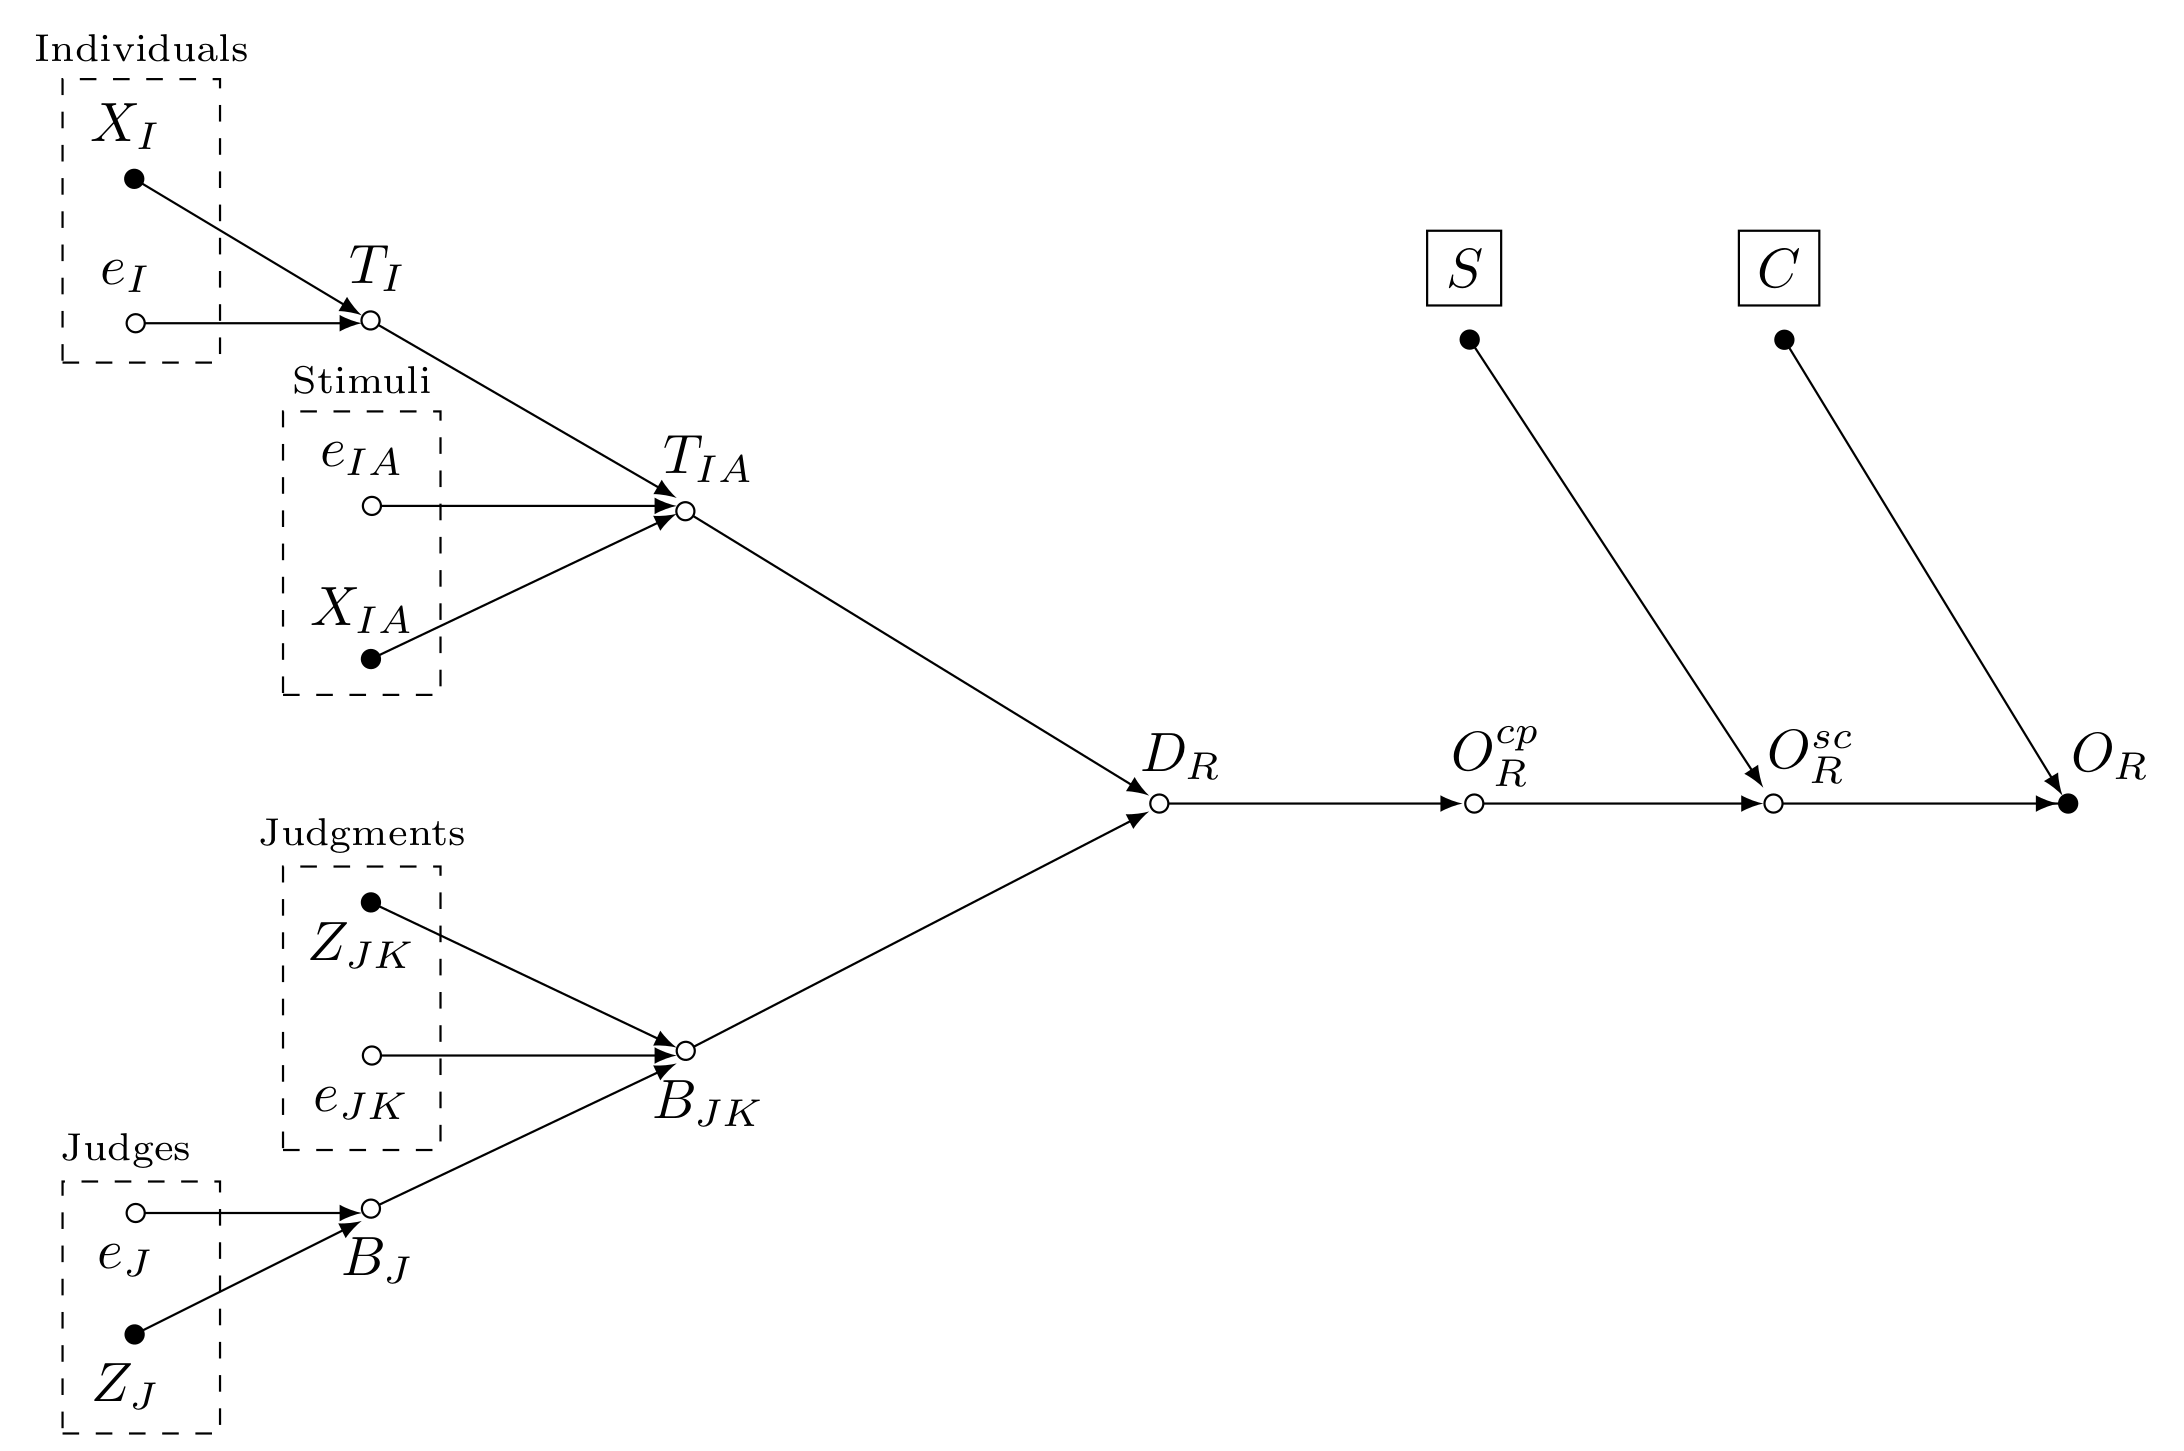
\includegraphics[width=1\linewidth,height=\textheight,keepaspectratio]{./images/png/CJ_TM_14.png}

}

\subcaption{\label{fig-cj14_dag}DAG}

\end{minipage}%

\caption{\label{fig-cj14}Sample-comparison model, final vectorized form}

\end{figure}%

However, because CJ experiments rarely use the exhaustive pairing of
sampled judges, stimuli, and individuals--due to concerns about the
practical feasibility of the comparison task
\citep{Boonen_et_al_2020}--a realistic scenario must also account for
judges comparing only specific stimuli from certain individuals.

\subsubsection{The comparison
mechanism}\label{sec-theory-theoretical_SC2}

As in the previous section, we begin defining the \emph{comparison
mechanism} using the binary vector variable \(C\) to facilitate the
interpretation of the sample-comparison model (see equation
(\ref{eq-mat27})). The vector contains \(n\) elements corresponding to
the number of rows in the \(R\) matrix, with each element
\(c_{(i,a,h,b,j,k)}\) being a binary value indicating the presence or
absence of data rows in \(R\), a definition similar to that of \(S\) in
equation (\ref{eq-mat26}).
\begin{equation}\phantomsection\label{eq-mat27}{
C = \begin{bmatrix}
c_{(1,1,1,2,1,1)} \\
\vdots \\
c_{(1,1,1,2,1,n_{K})} \\
\vdots \\
c_{(i,a,h,b,j,k)} \\
\vdots \\
c_{(n_{I},n_{A}-1,n_{I},n_{A},n_{J},1)} \\
\vdots \\
c_{(n_{I},n_{A}-1,n_{I},n_{A},n_{J},1)}
\end{bmatrix}
}\end{equation}

The DAG~\ref{fig-cj14_dag} also integrates the comparison mechanism
\(C\) into the conceptual-population model, which ultimately derives the
final comparative outcome \(O_{R}\). First, it shows the
sample-comparison outcome \(O^{sc}_{R}\) as unobserved, highlighting
that researchers cannot directly access this outcome due to the
comparison mechanism. Second, it depicts the \emph{comparison mechanism}
\(C\) as a causal factor influencing the final comparative outcome
\(O_{R}\). As with the sampling mechanism, a square encloses \(C\) to
indicate that it is a conditioned variable--that is, one that determines
\emph{which repeated judgments the subset of judges makes for the subset
of stimuli produced by the sampled individuals}. In essence, \(C\)
reflects the assumption that judges \emph{do not} perform all possible
repeated judgments for the selected stimuli. Instead, they carry out a
``sufficient number of comparisons'' \(n_{C}\) to allow for accurate
estimation of the proportion \(P(B>A)\) for each stimulus pair
\citep[pp.~267]{Thurstone_1927b}.

Notably, DAG~\ref{fig-cj14_dag} shows that \(C\) is independent of all
other variables in the model. This independence implies that the
conceptual model represented by the DAG applies exclusively to Random
Allocation Comparative Designs \citep{Bramley_2015} or Incomplete Block
Designs \citep{Lawson_2015}. In these designs, every repeated judgment
has an equal probability of being included in the sample.

\begin{figure}[H]

\begin{minipage}{\linewidth}

\centering{

\[
\begin{aligned}
  O_{R} & := f_{O}(D_{R}, S, C) \\
  D_{R} & := f_{D}(T_{IA}, B_{JK}) \\
  T_{IA} & := f_{T}(T_{I}, X_{IA}, e_{IA}) \\
  T_{I} & := f_{T}(X_{I}, e_{I}) \\
  B_{JK} & := f_{B}(B_{J}, Z_{JK}, e_{JK}) \\
  B_{J} & := f_{B}(Z_{J}, e_{J}) \\
  e_{I} & \:\bot\:\{ e_{J}, e_{IA}, e_{JK} \} \\
  e_{J} & \:\bot\:\{ e_{IA}, e_{JK} \} \\
  e_{IA} & \:\bot\:e_{JK} 
\end{aligned}
\]

}

\subcaption{\label{fig-cj15_scm}SCM}

\end{minipage}%
\newline
\begin{minipage}{\linewidth}

\centering{

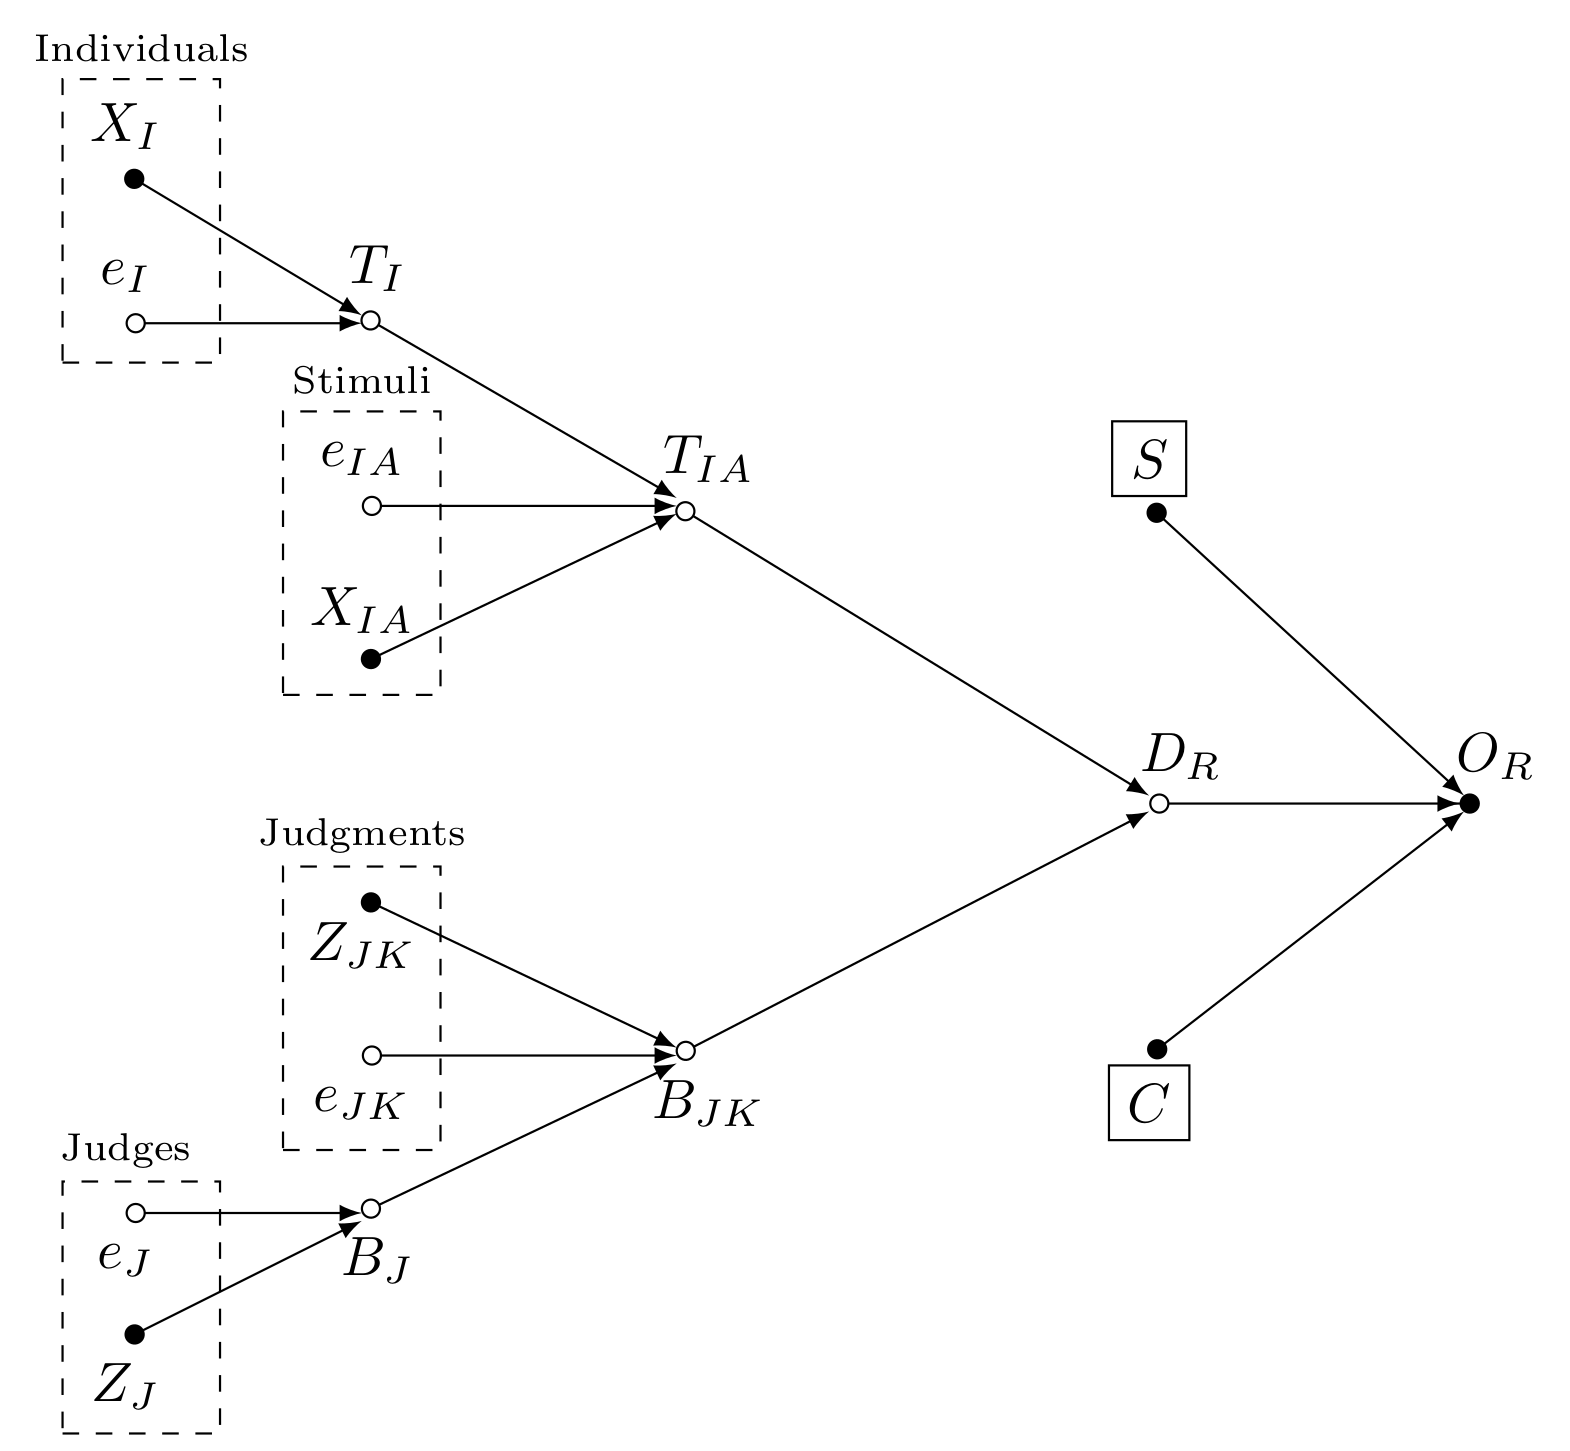
\includegraphics[width=0.72\linewidth,height=\textheight,keepaspectratio]{./images/png/CJ_TM_15.png}

}

\subcaption{\label{fig-cj15_dag}DAG}

\end{minipage}%

\caption{\label{fig-cj15}Comparative judgment model}

\end{figure}%

Finally, without loss of generality, researchers can reformulate the
sample-comparison model in Figure~\ref{fig-cj14} into the equivalent
form shown in Figure~\ref{fig-cj15}. This reformulation rests on two
principles. First, because the sampling and comparison mechanism vectors
\(S\) and \(C\) are binary, researchers can integrate them into the
model using element-wise products. This approach eliminates the need to
define the structural equations \(f_{S}\) and \(f_{C}\). Second, since
only the final comparative outcome \(O_{R}\) is observed, it is standard
to assume that the distribution of the conceptual-population outcome
\(O^{cp}_{R}\), defined by the structural equation \(f_{O}\), also
applies to this outcome. This assumption removes the necessity of
describing the unobserved outcomes \(O^{cp}_{R}\) and \(O^{sc}_{R}\).

In summary, extending Thurstone's general form allows researchers to
address issues with the BTL model, such as accounting for judge biases
(see Section~\ref{sec-theory-issue1b}), the hierarchical structure of
stimuli (see Section~\ref{sec-theory-issue1b}), and measurement error in
trait estimation and hypothesis testing (see
Section~\ref{sec-theory-issue2}). However, it does not address concerns
about stimuli' equal dispersions discussed in
Section~\ref{sec-theory-issue1a}. Since this issue involves statistical
assumptions regarding the discriminal process distribution, it requires
a statistical model, which we develop in the next section.

\section{Abandoning the BTL model}\label{sec-statistical}

Researchers can easily derive a statistical model to address violations
of the equal dispersion assumption in CJ experiments (see
Section~\ref{sec-theory-issue1a}) using only SCM~\ref{fig-cj15_scm}.
This derivation is possible because the structural equations \(F\)
encode probabilistic information \citep{Pearl_et_al_2016}, which
researchers can replace with suitable probabilistic assumptions. As a
starting point, given the dichotomous nature of CJ outcomes,
model~\ref{fig-cj16_stat} assumes that \(O_{R}\) follows a Bernoulli
distribution\footnote{The binomial distribution--including its special
  case, the Bernoulli distribution-- represent a maximum entropy
  distribution for binary events \citep[pp.~34]{McElreath_2020}. This
  means that when only two un-ordered outcomes are possible, and the
  expected numbers of each type of event are assumed to be constant,
  then the binomial distribution is the one that is most consistent with
  these constraints \citep[pp.~310]{McElreath_2020}. For a detailed
  discussion of the binomial as a maximum entropy distribution, see
  \citet[chap.~10.1.2]{McElreath_2020}.}.

Next, following the conventions of Generalized Linear Latent And Mixed
Models (GLLAMMs)
\citep{Rabe_et_al_2004a, Skrondal_et_al_2004a, Rabe_et_al_2012b}, the
model links the observed outcome to the latent discriminal difference
vector \(D_{R}\) using an inverse-logit function:
\(\text{inv\_logit}(x) = 1/(1 + \exp(-x))\). Notice that the sampling
and comparison mechanisms, \(S\) and \(C\), act as element-wise
multipliers of \(D_{R}\) (denoted by the symbol \(\odot\)), directly
incorporating key assessment design features relevant to CJ experiments
into the statistical formulation. Researchers can omit these vectors
when only the observed CJ sample is available.

\begin{figure}[H]

\begin{minipage}{0.50\linewidth}

\centering{

\[
\begin{aligned}
  O_{R} & \overset{iid}{\sim} \text{Bernoulli} \left[ \text{inv\_logit}( D_{R} \odot S \odot C ) \right] \\
  D_{R} & = \left( T_{IA}[i,a] - T_{IA}[h,b] \right) + B_{JK}[j,k] \\
  T_{IA} & = T_{I} + \beta_{XA} X_{IA} + e_{IA} \\
  T_{I} & = \beta_{XI} X_{I} + e_{I} \\
  B_{JK} & = B_{J} + \beta_{ZK} Z_{JK} + e_{JK} \\
  B_{J} & = \beta_{ZJ} Z_{J} + e_{J} \\
  e_{I} & \overset{iid}{\sim} \text{Normal}(0,s_{XI}) \\
  e_{J} & \overset{iid}{\sim} \text{Normal}(0,s_{ZJ}) \\
  e_{IA} & \overset{iid}{\sim} \text{Normal}(0, p_{IA}) \\  
  e_{JK} & \overset{iid}{\sim} \text{Normal}(0, p_{JK})
\end{aligned}
\]

}

\subcaption{\label{fig-cj16_stat}Statistical model}

\end{minipage}%
%
\begin{minipage}{0.50\linewidth}

\centering{

\[
\begin{aligned}
  O_{R} & := f_{O}(D_{R}, S, C) \\
  D_{R} & := f_{D}(T_{IA}, B_{JK}) \\
  T_{IA} & := f_{T}(T_{I}, X_{IA}, e_{IA}) \\
  T_{I} & := f_{T}(X_{I}, e_{I}) \\
  B_{JK} & := f_{B}(B_{J}, Z_{JK}, e_{JK}) \\
  B_{J} & := f_{B}(Z_{J}, e_{J}) \\
  e_{I} & \:\bot\:\{ e_{J}, e_{IA}, e_{JK} \} \\
  e_{J} & \:\bot\:\{ e_{IA}, e_{JK} \} \\
  e_{IA} & \:\bot\:e_{JK} 
\end{aligned}
\]

}

\subcaption{\label{fig-cj16_scm}SCM~\ref{fig-cj15_scm}}

\end{minipage}%

\caption{\label{fig-cj16}Comparative judgment model, SCM and statistical
model assuming different discriminal dispersions for the student's
traits}

\end{figure}%

Then, model~\ref{fig-cj16_stat} defines \(D_{R}\) as the difference
between the discriminal processes of two texts, \(T_{IA}[i, a]\) and
\(T_{IA}[h, b]\), which represent their underlying written-quality
trait. This difference also includes the corresponding repeated judge
biases, \(B_{JK}[j, k]\). Note that if we assume that \(B_{JK}[j,k]\)
reflects the difference in stimulus-specific biases, i.e.,
\(B_{JK}[j,k] = B_{JK}[i,a,j,k] - B_{JK}[h,b,j,k]\), then we can
re-write the discriminal difference as:
\begin{equation}\phantomsection\label{eq-mat51}{
\begin{aligned}
D_{R} &= \left( T_{IA}[i,a] - T_{IA}[h,b] \right) + B_{JK}[j,k] ] \\
&= \left( T_{IA}[i, a] + B_{JK}[i, a, j, k] \right) - \left( T_{IA}[h, b] + B_{JK}[h, b, j, k] \right) \\
& = T^{*}_{IA}[i,a] - T^{*}_{IA}[h,b]
\end{aligned}
}\end{equation} This formulation reveals that the discriminal difference
captures a \emph{pure interaction effect}, in which neither the texts'
discriminal processes nor the judges' biases alone determine the
outcome, but their interaction does \citep{Attia_et_al_2022}. In simple
terms, the discriminal processes of the stimuli become an observable
outcome only through the judges' perceptions (biases). For clarity, the
square brackets in \(D_{R}\) only indicate the relevant indices within
each trait vector; they do not represent any data subsetting.

Next, the model defines \(T_{IA}\) as a linear combination of the
students' underlying writing-quality traits \(T_{I}\), the effects of
relevant text-related variables \(\beta_{XA}X_{IA}\) (e.g., text
length), and the texts' idiosyncratic errors \(e_{IA}\). The model
assumes that each element of \(e_{IA}\) is independent and identically
distributed \((iid)\) according to a Normal distribution, with a mean of
zero and a standard deviation \(p_{IA}\), defined as a proportion of
\(1\). This standardization establishes the scale of the latent trait,
as it is required by latent variable models \citep{Depaoli_2021}.

Additionally, the model defines \(T_{I}\) as a linear combination of the
effects of relevant student-related variables, \(\beta_{XI} X_{I}\), and
students' idiosyncratic errors, \(e_{I}\). As before, each element of
\(e_{I}\) is \(iid\) following a Normal distribution with a mean of
zero. However, the standard deviation, \(s_{XI}\), varies depending on
the teaching method to which each student belongs. Given the example in
Section~\ref{sec-theoretical}, where the teaching method
\(X_{I} = 1,2\), the model sets the following constraint to anchor the
scale of the latent trait \citep{Depaoli_2021}:
\(\sum_{g=1}^{2} s_{XI}[g]/2 = 1\) This constraint effectively addresses
concerns about the equal dispersion assumption raised in
Section~\ref{sec-theory-issue1a}.

Similarly, the model defines \(B_{JK}\) as a linear combination of the
judges' individual bias \(B_{J}\), the effects of relevant
judgment-related variables \(\beta_{ZK}Z_{JK}\) (e.g., the number of
judgments a judge makes), and judgment-specific idiosyncratic errors
\(e_{JK}\). The model assumes that each element of \(e_{JK}\) is \(iid\)
according to a Normal distribution, with a mean of zero and a standard
deviation \(p_{JK}\), defined as a proportion of \(1\), to anchor the
scale of the latent trait \citep{Depaoli_2021}.

The model also defines \(B_{J}\) as a linear combination of the effects
of relevant judge-level variables \(\beta_{ZJ}Z_{J}\) (e.g., judgment
expertise) and judge-specific idiosyncratic errors \(e_{J}\). Each
element of \(e_{J}\) is likewise assumed to be \(iid\) Normal with mean
zero and a standard deviation \(s_{ZJ}\) that depends on the groups to
which each judge belongs. For instance, if \(Z_{J} = 1, \dots, 3\)
represents three groups of judges with varying expertise, the model
imposes the constraint \(\sum_{g=1}^{3} s_{ZJ}[g]/3 = 1\) to fix the
scale of the latent trait \citep{Depaoli_2021}.

Finally, we apply \emph{Bayesian inference methods} to turn
model~\ref{fig-cj16_stat} into a practical statistical tool for
analyzing paired comparison data. The \textbf{Declarations} section of
this document provides a link to this model, along with an alternative
specification that assumes equal discriminal dispersions. We implemented
both models in \texttt{Stan} \citep[version \(2.26.1\),][]{Stan_2020}.

\section{Discussion}\label{sec-discussion}

\subsection{Findings}\label{sec-discussion-finding}

\subsection{Limitations and further
research}\label{sec-discussion-limitations}

\section{Conclusion}\label{sec-conclusion}

\newpage{}

\section*{Declarations}\label{declarations}
\addcontentsline{toc}{section}{Declarations}

\textbf{Funding:} The Research Fund (BOF) of the University of Antwerp
funded this project.

\textbf{Financial interests:} The authors declare no relevant financial
interests.

\textbf{Non-financial interests:} The authors declare no relevant
non-financial interests.

\textbf{Ethics approval:} The University of Antwerp Research Ethics
Committee confirmed that this study does not require ethical approval.

\textbf{Consent to participate:} Not applicable

\textbf{Consent for publication:} All authors have read and approved the
final version of the manuscript for publication.

\textbf{Data availability:} This study did not use any data.

\textbf{Materials and code availability:} The \texttt{CODE\ LINK}
section at the top of the digital document located at:
\url{https://jriveraespejo.github.io/paper2_manuscript/} provides access
to all materials and code.

\textbf{AI-assisted technologies in the writing process:} The authors
used various AI-based language tools to refine phrasing, optimize
wording, and enhance clarity and coherence throughout the manuscript.
They take full responsibility for the final content of the publication.

\textbf{CRediT authorship contribution statement:}
\emph{Conceptualization:} J.M.R.E, T.vD., S.DM., and S.G.;
\emph{Methodology:} J.M.R.E, T.vD., and S.DM.; \emph{Software:}
J.M.R.E.; \emph{Validation:} J.M.R.E.; \emph{Formal Analysis:} J.M.R.E.;
\emph{Investigation:} J.M.R.E; \emph{Resources:} T.vD. and S.DM.;
\emph{Data curation:} J.M.R.E.; \emph{Writing - original draft:}
J.M.R.E.; \emph{Writing - review and editing:} T.vD., S.DM., and S.G.;
\emph{Visualization:} J.M.R.E.; \emph{Supervision:} S.G. and S.DM.;
\emph{Project administration:} S.G. and S.DM.; \emph{Funding
acquisition:} S.G. and S.DM.

\newpage{}

\section{Appendix}\label{sec-appendix}

\subsection{Statistical and Causal inference}\label{sec-appendixB}

This section introduces fundamental statistical and causal inference
concepts necessary for understanding the core theoretical principles
described in this document. It does not, however, offer a comprehensive
overview of causal inference methods. Readers seeking more in-depth
understanding may wish to explore introductory papers such as
\citet{Pearl_2010}, \citet{Rohrer_2018}, \citet{Pearl_2019}, and
\citet{Cinelli_et_al_2020}. They may also find it helpful to consult
introductory books like \citet{Pearl_et_al_2018}, \citet{Neal_2020}, and
\citet{McElreath_2020}. For more advanced study, readers may refer to
seminal intermediate papers such as \citet{Neyman_et_al_1923},
\citet{Rubin_1974}, \citet{Spirtes_et_al_1991}, and \citet{Sekhon_2009},
as well as books such as \citet{Pearl_2009}, \citet{Morgan_et_al_2014},
and \citet{Hernan_et_al_2020}.

\subsubsection{Empirical research and randomized
experiments}\label{sec-appendixB1}

Empirical research uses evidence from observation and experimentation to
address real-world challenges. In this context, researchers typically
formulate their research questions as \emph{estimands} or \emph{targets
of inference}, i.e., the specific quantities they seek to determine
\citep{Everitt_et_al_2010}. For instance, researchers might be
interested in answering the following question: ``To what extent do
different teaching methods \((T)\) influence students' ability to
produce high-quality written texts \((Y)\)?'' To investigate this,
researchers could randomly assign students to two groups, each exposed
to a different teaching method \((T_{i} = \{1,2\})\). Then, they would
perform pairwise comparisons, generating a dichotomous outcome
\((Y_{i} = \{0,1\})\) showing which student exhibits more of the
ability. In this scenario, the research question can be rephrased as the
estimand, ``\emph{On average}, is there a difference in the ability to
produce high-quality written texts between the two groups of students?''
and this estimand can be mathematically represented by the random
associational quantity in Equation~\ref{eq-group_diff}, where
\(E[\cdot]\) denotes the expected value.

\begin{equation}\phantomsection\label{eq-group_diff}{
E[Y_{i} \:|\:T_{i}=1] - E[Y_{i} \:|\:T_{i}=2]
}\end{equation}

Researchers then proceed to identify the estimands.
\emph{Identification} determines whether an estimator can accurately
compute the estimand based solely on its assumptions, regardless of
random variability \citep[pp.~4]{Schuessler_et_al_2023}. An
\emph{estimator} refers to a method or function that transforms data
into an estimate \citep{Neal_2020}. \emph{Estimates} are numerical
values that approximate the estimand derived through the process of
\emph{estimation}, which integrates data with an estimator
\citep{Everitt_et_al_2010}. The Identification-Estimation flowchart
\citep{McElreath_2020, Neal_2020}, shown in Figure~\ref{fig-IEflow},
visually represents the transition from estimands to estimates.

\begin{figure}

\centering{

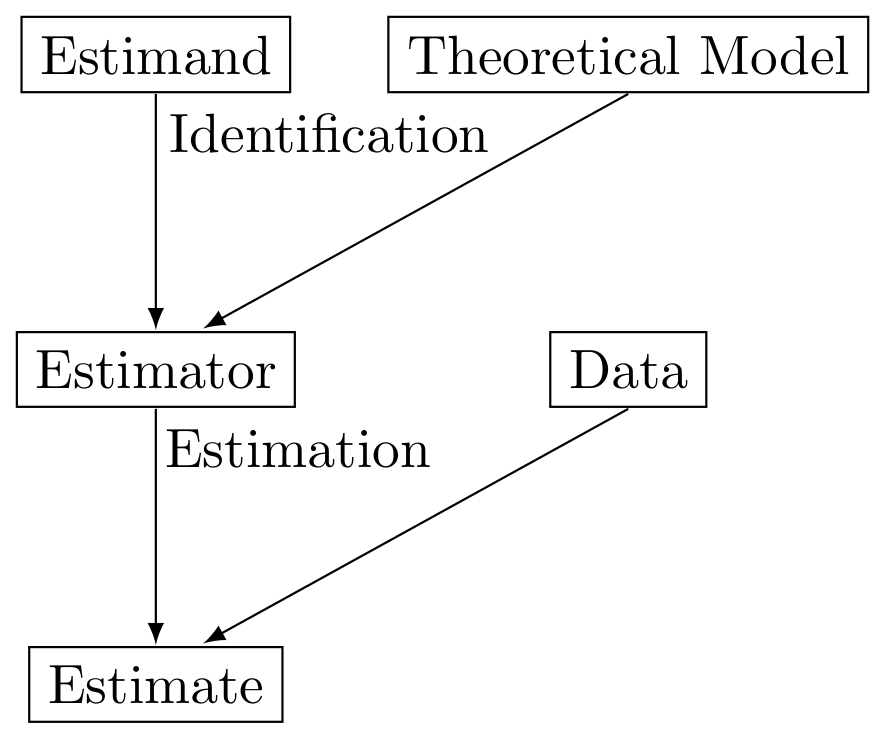
\includegraphics[width=0.35\linewidth,height=\textheight,keepaspectratio]{images/png/IEflow.png}

}

\caption{\label{fig-IEflow}Identification-Estimation flowchart.
Extracted and slightly modified from \citet[pp.~32]{Neal_2020}}

\end{figure}%

Identification is a necessary condition to ensure \emph{consistent}
estimators. An estimator achieves \emph{consistency} when it converges
to the ``true'' value of an estimand as the data size approaches
infinity \citep{Everitt_et_al_2010}. Without identification, researchers
cannot achieve consistency, even with ``infinite'' and error-free data.
As a result, deriving meaningful insights about an estimand from finite
data becomes impossible \citep[pp.~5]{Schuessler_et_al_2023}. Therefore,
to ensure accurate and reliable estimates, researchers prioritize
estimators with desirable identification properties. For instance, the
Z-test is a widely used estimator for comparing group proportions,
yielding accurate estimates when its underlying assumptions are
satisfied \citep{Kanji_2006}. Furthermore, researchers can interpret
estimates from the Z-test as causal, provided the data is collected
through a randomized experiment.

Randomized experiments are widely recognized as the gold standard in
evidence-based science \citep{Hariton_et_al_2018, Hansson_2014}. This
recognition stems from their ability to enable researchers interpret
associational estimates as causal. They achieve this by ensuring data,
and by extension an estimator, satisfies several key identification
properties, such as common support, no interference, and consistency
\citep{Morgan_et_al_2014, Neal_2020}. The most critical property,
however, is the elimination of confounding. \emph{Confounding} occurs
when an external variable \(X\) simultaneously influences the outcome
\(Y\) and the variable of interest \(T\), resulting in spurious
associations \citep{Everitt_et_al_2010}. Randomization addresses this
issue by decoupling the association between the intervention allocation
\(T\) from any other variable \(X\)
\citep{Morgan_et_al_2014, Neal_2020}.

Nevertheless, researchers often face constraints that limit their
ability to conduct randomized experiments. These constraints include
ethical concerns, such as the assignment of individuals to potentially
harmful interventions, and practical limitations, such as the
infeasibility of, for example, assigning individuals to genetic
modifications or physical impairments \citep{Neal_2020}. In these cases,
causal inference offers a valuable alternative for generating causal
estimates and understanding the mechanisms underlying specific data. In
addition, the framework can provide significant theoretical insights
that can enhance the design of experimental and observational studies
\citep{McElreath_2020}.

\subsubsection{Identification under causal
inference}\label{sec-appendixB2}

Unlike classical statistical modeling, which focuses primarily on
summarizing data and inferring associations, the \emph{causal inference}
framework is designed to identify causes and estimate their effects
using data \citep{Shaughnessy_et_al_2010, Neal_2020}. The framework uses
rigorous mathematical techniques to address the \emph{fundamental
problem of causality}
\citep{Pearl_2009, Pearl_et_al_2016, Morgan_et_al_2014}. This problem
revolves around the question, ``What would have happened `in the world'
under different circumstances?'' This question introduces the concept of
counterfactuals, which are instrumental in defining and identifying
causal effects.

\emph{Counterfactuals} are hypothetical scenarios that are
\emph{contrary to fact}, where alternative outcomes resulting from a
given cause are neither observed nor observable
\citep{Neal_2020, Counterfactual_2024}. The structural approach to
causal inference \citep{Pearl_2009, Pearl_et_al_2016} provides a formal
framework for defining counterfactuals. For instance, in the scenario
described in Section~\ref{sec-appendixB1}, the approach begins by
defining the \emph{individual causal effect} (ICE) as the difference
between each student's potential outcomes, as in Equation~\ref{eq-ICE}.

\begin{equation}\phantomsection\label{eq-ICE}{
\tau_{i} = Y_{i} \:|\:do(T_{i}=1) - Y_{i} \:|\:do(T_{i}=2)
}\end{equation}

where \(do(T_{i}=t)\) represents the intervention operator,
\(Y_{i} \:|\:do(T_{i}=1)\) represents the potential outcome under
intervention \(T_{i}=1\), and \(Y_{i} \:|\:do(T_{i}=1)\) represents the
potential outcome under intervention \(T_{i}=2\). Here, an
\emph{intervention} involves assigning a constant value to the treatment
variable for each student's potential outcomes. Note that if a student
is assigned to intervention \(T_{i}=1\), the potential outcome under
\(T_{i}=2\) becomes a counterfactual, as it is no longer observed nor
observable. To address this challenge, the structural approach extends
the ICE to the \emph{average causal effect} (ACE,
Equation~\ref{eq-ACE}), representing the average difference between the
students' observed potential outcomes and their counterfactual
counterparts.

\begin{equation}\phantomsection\label{eq-ACE}{
\begin{aligned}
\tau & = E[\tau_{i}] \\
  & = E[Y_{i} \:|\:do(T_{i}=1)]- E[Y_{i} \:|\:do(T_{i}=2)]
\end{aligned}
}\end{equation}

Even though counterfactuals are unobservable, researchers can still
identify the ACE from associational estimates by leveraging the
structural approach. The approach identifies the ACE by statistically
conditioning data on a \emph{sufficient adjustment set} of variables
\(X\) \citep{Pearl_2009, Pearl_et_al_2016, Morgan_et_al_2014}. This
\emph{sufficient} set (potentially empty) must block all non-causal
paths between \(T\) to \(Y\) without opening new ones. When such a set
exists, then \(T\) and \(Y\) are \emph{d-separated} by \(X\)
(\(T \:\bot\:Y \:|\:X\)) \citep{Pearl_2009}, and \(X\) satisfies the
\emph{backdoor criterion} \citep[pp 37]{Neal_2020}. Here,
\emph{conditioning} describes the process of restricting the focus to
the subset of the population defined by the conditioning variable
\citep[pp.~32]{Neal_2020} (see Equation~\ref{eq-CACE}).

Conditioning on a sufficient adjustment set enables researchers to
estimate the ACE, even when the data comes from an observational study.
This process is feasible because such conditioning ensures that the ACE
estimator satisfies several critical properties, including confounding
elimination \citep{Morgan_et_al_2014}. Naturally, the validity of claims
about the causal effects of \(T\) on \(Y\) now hinges on the assumption
that \(X\) serves as a sufficient adjustment set. However, as
\citet[pp.~150]{Kohler_et_al_2019} noted, drawing conclusions about the
real world from observed data inevitably requires assumptions. This
requirement holds true for both observational and experimental data.

For instance, if researchers cannot conduct the randomized experiments
described in Section~\ref{sec-appendixB1} and must instead rely on
observational data, they can still identify the ACE as long as an
observed variable \(X\), such as the socio-economic status of the
school, satisfies the backdoor criterion. Under these circumstances,
researchers first identify the \emph{conditional average causal effect}
(CACE, Equation~\ref{eq-CACE})

\begin{equation}\phantomsection\label{eq-CACE}{
CACE_{t} = E[Y_{i} \:|\:T_{i}=t, X]
}\end{equation}

From the CACE, researchers can identify the ACE from associational
quantities as in Equation~\ref{eq-mACE1}. This identification process is
commonly known as the \emph{backdoor adjustment}. Here, \(E_{X}[\cdot]\)
represents the marginal expected value over \(X\)
\citep{Morgan_et_al_2014}.

\begin{equation}\phantomsection\label{eq-mACE1}{
\begin{aligned}
  \tau & = E[Y_{i} \:|\:do(T_{i}=1)]- E[Y_{i} \:|\:do(T_{i}=2)] \\
  & = E_{X}[CACE_{1} - CACE_{2}] \\
  & = E_{X}\left[ E[Y_{i} \:|\:T_{i}=1, X] - E[Y_{i} \:|\:T_{i}=2, X] \right]
\end{aligned}
}\end{equation}

Notably, the approach extends the ACE identification for a continuous
variable \(T\) as in Equation~\ref{eq-mACE_cont}, ensuring broad
applicability across different causal scenarios
\citep[pp.~45]{Neal_2020}

\begin{equation}\phantomsection\label{eq-mACE_cont}{
\begin{aligned}
  \tau &= E[Y_{i} \:|\:do(T_{i}=t)] \\
  & = d E_{X}\left[ E[Y_{i} \:|\:T_{i}=t, X]\right]/ dt
  \end{aligned}
}\end{equation}

\subsubsection{Diving into the specifics}\label{sec-appendixB3}

The structural approach to causal inference uses SCMs and DAGs to
formally and graphically represent the presumed causal structure
underlying the ACE
\citep{Pearl_2009, Pearl_et_al_2016, Gross_et_al_2018, Neal_2020}.
Essentially, these tools serve as \emph{conceptual (theoretical) models}
on which identification analysis rests
\citep[pp.~4]{Schuessler_et_al_2023}. Thus, using these tools,
researchers can determine which statistical models can identify (ACE,
CACE, or other), assuming the depicted causal structure is correct
\citep{McElreath_2020}, thus enabling valid causal inference.
Figure~\ref{fig-IEflow} shows the role of theoretical models in the
inference process.

SCMs and DAGs support identification analysis through two key
advantages. First, regardless of complexity, they can represent various
causal structures using only five fundamental building blocks
\citep{Neal_2020, McElreath_2020}. This feature allows researchers to
decompose complex structures into manageable components, facilitating
their analysis \citep{McElreath_2020}. Second, they depict causal
relationships in a non-parametric and fully interactive way. This
flexibility enables feasible ACE identification strategies without
defining the variables' data types, the functional form between them, or
their parameters \citep[pp.~35]{Pearl_et_al_2016}.

Thus, Section~\ref{sec-appendixB31} and Section~\ref{sec-appendixB32}
elaborate on the first advantage, while Section~\ref{sec-appendixB32}
and Section~\ref{sec-appendixB33} do so for the second. Finally,
Section~\ref{sec-appendixB34} explains how researchers use SCMs and DAGs
alongside Bayesian inference methods in the estimation process.

\paragraph{The five fundamental block for SCMs and
DAGs}\label{sec-appendixB31}

Figures \ref{fig-dags_scms1}, \ref{fig-dags_scms2},
\ref{fig-dags_scms3}, \ref{fig-dags_scms4}, and \ref{fig-dags_scms5}
display the five fundamental building blocks for SCMs and DAGs. The left
panels of the figures show the formal mathematical models, represented
by the SCMs, defined in terms of a set of \emph{endogenous} variables
\(V=\{X_{1},X_{2},X_{3}\}\), a set of \emph{exogenous} variables
\(E=\{e_{X1},e_{X2},e_{X3}\}\), and a set of functions
\(F=\{f_{X1},f_{X2},f_{X3}\}\) \citep{Pearl_2009, Cinelli_et_al_2020}.
Endogenous variables are those whose causal mechanisms a researcher
chooses to model \citep{Neal_2020}. In contrast, exogenous variables
represent \emph{errors} or \emph{disturbances} arising from omitted
factors that the investigator chooses not to model explicitly
\citep[pp.~27,68]{Pearl_2009}. Lastly, the functions, referred to as
\emph{structural equations}, express the endogenous variables as
non-parametric functions of other variables. These functions use the
symbol `\(:=\)' to denote the asymmetrical causal dependence of the
variables and the symbol `\(\:\bot\:\)' to represent
\emph{d-separation}, a concept akin to (conditional) independence.

Notably, every SCM has an associated DAG
\citep{Pearl_et_al_2016, Cinelli_et_al_2020}. The right panels of the
figures display these DAGs. A DAG is a graph consisting of nodes
connected by edges, where the nodes represent random variables. The term
\emph{directed} means that the edges extend from one node to another,
with arrows indicating the direction of causal influence. The term
\emph{acyclic} implies that the causal influences do not form loops,
ensuring the influences do not cycle back on themselves
\citep{McElreath_2020}. DAGs represent observed variables as solid black
circles, while they use open circles for unobserved (latent) variables
\citep{Morgan_et_al_2014}. Although the \emph{standard representation}
of DAGs typically omits exogenous variables for simplicity, the
\emph{magnified representation} depicted in the figures offers one key
advantage: including exogenous variables can help researchers highlight
potential issues related to conditioning and confounding
\citep{Cinelli_et_al_2020}.

\begin{figure}[H]

\begin{minipage}{0.50\linewidth}

\centering{

\[
\begin{aligned}
  X_{1} & := f_{X1}(e_{X1}) \\
  X_{3} & := f_{X3}(e_{X3}) \\
  e_{X1} & \:\bot\:e_{X3}
\end{aligned}
\]

}

\subcaption{\label{fig-scm_bb1}SCM}

\end{minipage}%
%
\begin{minipage}{0.50\linewidth}

\centering{

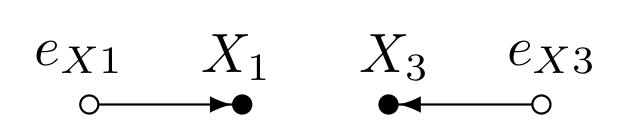
\includegraphics[width=0.54\linewidth,height=\textheight,keepaspectratio]{images/png/mdag_bb1.png}

}

\subcaption{\label{fig-mdag_bb1}DAG}

\end{minipage}%

\caption{\label{fig-dags_scms1}Two unconnected nodes}

\end{figure}%

\begin{figure}[H]

\begin{minipage}{0.50\linewidth}

\centering{

\[
\begin{aligned}
  X_{1} & := f_{X1}(e_{X1}) \\
  X_{3} & := f_{X3}(X_{1},e_{X3}) \\
  e_{X1} & \:\bot\:e_{X3}
\end{aligned}
\]

}

\subcaption{\label{fig-scm_bb2}SCM}

\end{minipage}%
%
\begin{minipage}{0.50\linewidth}

\centering{

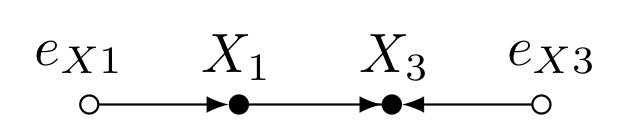
\includegraphics[width=0.54\linewidth,height=\textheight,keepaspectratio]{images/png/mdag_bb2.png}

}

\subcaption{\label{fig-mdag_bb2}DAG}

\end{minipage}%

\caption{\label{fig-dags_scms2}Two connected nodes or descendant}

\end{figure}%

\begin{figure}[H]

\begin{minipage}{0.50\linewidth}

\centering{

\[
\begin{aligned}
  X_{1} & := f_{X1}(e_{X1}) \\
  X_{2} & := f_{X2}(X_{1},e_{X2}) \\
  X_{3} & := f_{X3}(X_{2},e_{X3}) \\
  e_{X1} & \:\bot\:e_{X2} \\
  e_{X1} & \:\bot\:e_{X3} \\
  e_{X2} & \:\bot\:e_{X3}
\end{aligned}
\]

}

\subcaption{\label{fig-scm_bb3}SCM}

\end{minipage}%
%
\begin{minipage}{0.50\linewidth}

\centering{

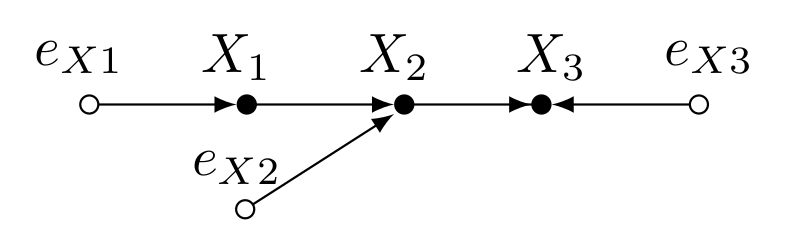
\includegraphics[width=0.65\linewidth,height=\textheight,keepaspectratio]{images/png/mdag_bb3.png}

}

\subcaption{\label{fig-mdag_bb3}DAG}

\end{minipage}%

\caption{\label{fig-dags_scms3}Chain or mediator}

\end{figure}%

\begin{figure}[H]

\begin{minipage}{0.50\linewidth}

\centering{

\[
\begin{aligned}
  X_{1} & := f_{X1}(X_{2},e_{X1}) \\
  X_{2} & := f_{X2}(e_{X2}) \\
  X_{3} & := f_{X3}(X_{2},e_{X3}) \\
  e_{X1} & \:\bot\:e_{X2} \\
  e_{X1} & \:\bot\:e_{X3} \\
  e_{X2} & \:\bot\:e_{X3}
\end{aligned}
\]

}

\subcaption{\label{fig-scm_bb4}SCM}

\end{minipage}%
%
\begin{minipage}{0.50\linewidth}

\centering{

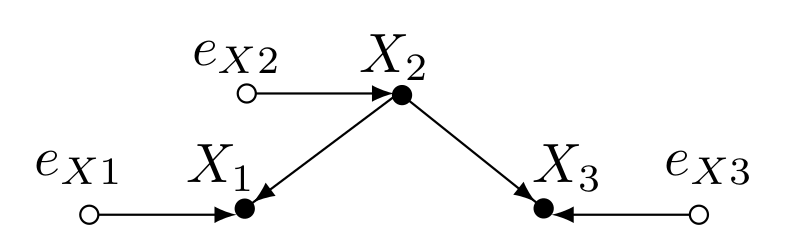
\includegraphics[width=0.65\linewidth,height=\textheight,keepaspectratio]{images/png/mdag_bb4.png}

}

\subcaption{\label{fig-mdag_bb4}DAG}

\end{minipage}%

\caption{\label{fig-dags_scms4}Fork or confounder}

\end{figure}%

\begin{figure}[H]

\begin{minipage}{0.50\linewidth}

\centering{

\[
\begin{aligned}
  X_{1} & := f_{X1}(e_{X1}) \\
  X_{2} & := f_{X2}(X_{1},X_{3},e_{X2}) \\
  X_{3} & := f_{X3}(e_{X3}) \\
  e_{X1} & \:\bot\:e_{X2} \\
  e_{X1} & \:\bot\:e_{X3} \\
  e_{X2} & \:\bot\:e_{X3}
\end{aligned}
\]

}

\subcaption{\label{fig-scm_bb5}SCM}

\end{minipage}%
%
\begin{minipage}{0.50\linewidth}

\centering{

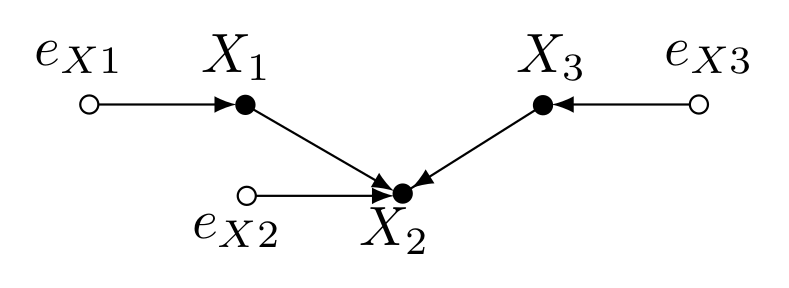
\includegraphics[width=0.65\linewidth,height=\textheight,keepaspectratio]{images/png/mdag_bb5.png}

}

\subcaption{\label{fig-mdag_bb5}DAG}

\end{minipage}%

\caption{\label{fig-dags_scms5}Collider or inmorality}

\end{figure}%

A careful examination of these building blocks highlights the
theoretical assumptions underlying their observed variables. SCM
\ref{fig-scm_bb1} and DAG \ref{fig-mdag_bb1} depict two unconnected
nodes, representing a scenario where variables \(X_{1}\) and \(X_{3}\)
are independent or not causally related. SCM \ref{fig-scm_bb2} and DAG
\ref{fig-mdag_bb2} illustrate two connected nodes, representing a
scenario where a \emph{parent} node \(X_{1}\) exerts a causal influence
on a \emph{child} node \(X_{3}\). In this setup, \(X_{3}\) is considered
a \emph{descendant} of \(X_{1}\). Additionally, \(X_{1}\) and \(X_{3}\)
are described as \emph{adjacent} because there is a \emph{direct path}
connecting them. SCM \ref{fig-scm_bb3} and DAG \ref{fig-mdag_bb3} depict
a \emph{chain}, where \(X_{1}\) influences \(X_{2}\), and \(X_{2}\)
influences \(X_{3}\). In this configuration, \(X_{1}\) is a parent node
of \(X_{2}\), which is a parent node of \(X_{3}\). This structure
creates a \emph{directed path} between \(X_{1}\) and \(X_{3}\).
Consequently, \(X_{1}\) is an \emph{ancestor} of \(X_{3}\), and
\(X_{2}\) fully \emph{mediates} the relationship between the two. SCM
\ref{fig-scm_bb4} and DAG \ref{fig-mdag_bb4} illustrate a \emph{fork},
where variables \(X_{1}\) and \(X_{3}\) are both influenced by
\(X_{2}\). Here, \(X_{2}\) is a parent node that \emph{confounds} the
relationship between \(X_{1}\) and \(X_{3}\). Finally, SCM
\ref{fig-scm_bb5} and DAG \ref{fig-mdag_bb5} show a \emph{collider},
where variables \(X_{1}\) and \(X_{3}\) are concurrent causes of
\(X_{2}\). In this configuration, \(X_{1}\) and \(X_{3}\) are not
causally related to each other but both influence \(X_{2}\) (an
\emph{inmorality}). Notably, all building blocks assume the errors are
independent of each other and from all other variables in the graph, as
evidenced by the pairwise relations \(e_{X1} \:\bot\:e_{X2}\),
\(e_{X1} \:\bot\:e_{X3}\), and \(e_{X2} \:\bot\:e_{X3}\).

Researchers can then use these building blocks to represent the scenario
outlined in Section~\ref{sec-appendixB2}. SCM \ref{fig-scm_example1} and
DAG \ref{fig-mdag_example1} depict the plausible causal structure for
this example. In this context, the variable \(X\) (socio-economic status
of the school) is thought to be a confounder in the relationship between
the teaching method \(T\) and the outcome \(Y\). The figures display
multiple descendant relationships such as \(X \rightarrow T\),
\(X \rightarrow Y\), and \(T \rightarrow Y\). They also highlight
unconnected node pairs, evident from the relationships
\(e_{T} \:\bot\:e_{X}\), \(e_{T} \:\bot\:e_{Y}\), and
\(e_{X} \:\bot\:e_{Y}\). Additional, the figures show one fork,
\(X \rightarrow \{T, Y\}\), and two colliders:
\(\{X, e_{T}\} \rightarrow T\) and \(\{X, T, e_{Y}\} \rightarrow Y\).

\begin{figure}

\begin{minipage}{0.50\linewidth}

\centering{

\[
\begin{aligned}
  X & := f_{X}(e_{X}) \\
  T & := f_{T}(X,e_{T}) \\
  Y & := f_{Y}(T,X,e_{Y}) \\
  e_{T} & \:\bot\:e_{X} \\
  e_{T} & \:\bot\:e_{Y} \\
  e_{X} & \:\bot\:e_{Y}
\end{aligned}
\]

}

\subcaption{\label{fig-scm_example1}SCM}

\end{minipage}%
%
\begin{minipage}{0.50\linewidth}

\centering{

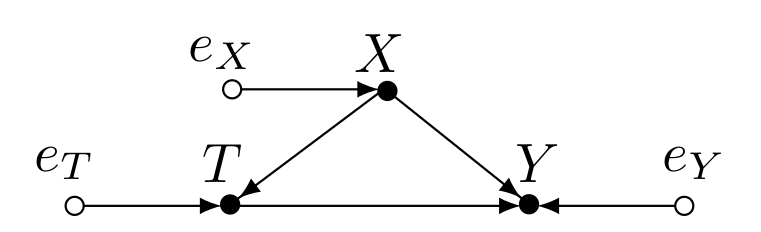
\includegraphics[width=0.65\linewidth,height=\textheight,keepaspectratio]{images/png/mdag_example1.png}

}

\subcaption{\label{fig-mdag_example1}DAG}

\end{minipage}%

\caption{\label{fig-example1}Plausible causal structure the scenario
outlined in Section~\ref{sec-appendixB2}.}

\end{figure}%

\paragraph{The probabilistic implications of these
blocks}\label{sec-appendixB32}

Beyond their graphical capabilities, SCMs and DAGs can encode the
probabilistic information embedded within a causal structure. They
achieve this encoding by relying on three fundamental assumptions: the
local Markov, the minimality, the causal edges assumption. The
\emph{local Markov assumption} encodes probabilistic independencies
between variables by declaring that nodes in a graph are independent of
all its non-descendants, given its parents \citep[pp.~20]{Neal_2020}.
Meanwhile, the \emph{minimality assumption} encodes probabilistic
dependencies among variables by stating that every pair of adjacent
nodes exhibits a dependency \citep[pp.~21]{Neal_2020}. Finally, the
\emph{causal edges assumption} encodes causal relationships between
variables by declaring that each parent node acts as a direct cause of
its children \citep[pp.~22]{Neal_2020}. Figure~\ref{fig-ACflow}
illustrates how these assumptions influence the statistical and causal
interpretations of graphs.

\begin{figure}

\centering{

\includegraphics[width=0.8\linewidth,height=\textheight,keepaspectratio]{images/png/ACflow.png}

}

\caption{\label{fig-ACflow}The flow of association and causation in
graphs. Extracted and slightly modified from \citet[pp.~31]{Neal_2020}}

\end{figure}%

A notable implication of the assumptions underlying the probabilistic
encoding is that any conceptual model described by an SCM and DAG can
represent the joint distribution of variables more efficiently
\citep[pp.~29]{Pearl_et_al_2016}. This expression takes the form of a
product of conditional probability distributions (CPDs) of the type
\(P(child \:|\:parents)\). This property is formally known as the
\emph{Bayesian Network factorization} (BNF,
Equation~\ref{eq-net_factor})
\citetext{\citealp[pp.~29]{Pearl_et_al_2016}; \citealp[pp.~21]{Neal_2020}}.
In this expression, \(pa(X_{i})\) denotes the set of variables that are
the parents of \(X_{i}\).
\begin{equation}\phantomsection\label{eq-net_factor}{
\begin{aligned}
P(X_{1}, X_{2}, \dots, X_{P}) & = X_{1} \cdot \prod^{P}_{p=2} P(X_{i} \:|\:X_{i-1}, \dots, X_{1}) & (\small{\text{by chain rule})}\\
& = X_{1} \cdot \prod^{P}_{p=2} P(X_{i} \:|\:pa(X_{i}) ) & (\small{\text{by BNF}})
\end{aligned}
}\end{equation}

This encoding enables researchers with conceptual (theoretical)
knowledge in the form of an SCM and DAG to predict patterns of
(in)dependencies in the data. As highlighted by
\citet[pp.~35]{Pearl_et_al_2016}, these predictions depend solely on the
structure of these conceptual models without requiring the quantitative
details of the equations or the distributions of the errors. Moreover,
once researchers observe empirical data, the patterns of
(in)dependencies in the data can provide significant insights into the
validity of the proposed conceptual model.

The five fundamental building blocks described in
Section~\ref{sec-appendixB31} clearly illustrate which (in)dependencies
can SMCs and DAGs predict. For instance, applying the BNF to the causal
structure shown in the SCM \ref{fig-scm_bb1} and DAG \ref{fig-mdag_bb1}
enables researchers to express the joint probability distribution of the
observed variables as \(P(X_{1}, X_{3}) = P(X_{1}) P(X_{3})\),
supporting the theoretical assumption that the observed variables
\(X_{1}\) and \(X_{3}\) are unconditionally independent
(\(X_{1} \:\bot\:X_{3}\)) \citep[pp.~24]{Neal_2020}. Conversely, when
\(X_{3}\) is unconditionally dependent on \(X_{1}\)
(\(X_{1} \:\not\bot\:X_{3}\)), as depicted in the SCM \ref{fig-scm_bb2}
and DAG \ref{fig-mdag_bb2}, the BNF express their joint probability
distribution as \(P(X_{1}, X_{3}) = P(X_{3} \:|\:X_{1}) P(X_{1})\).
Notably, these descriptions demonstrate the clear correspondence between
the structural equations illustrated in Section~\ref{sec-appendixB31}
and the CPDs.

Beyond the insights gained from two-node structures, researchers can
uncover more nuanced patterns of(in)dependencies from chains, forks, and
colliders. These (in)dependencies apply to any data set generated by a
causal model with those structures, regardless of the specific functions
attached to the SCM \citep[pp.~36]{Pearl_et_al_2016}. For instance,
applying the BNF to the chain structure depicted in the SCM
\ref{fig-scm_bb3} and DAG \ref{fig-mdag_bb3} allow researchers to
represent the joint distribution for the observed variables as
\(P(X_{1},X_{2},X_{3}) =\)
\(P(X_{1}) P(X_{2} \:|\:X_{1}) P(X_{3} \:|\:X_{2})\). This expression
implies that \(X_{1}\) and \(X_{3}\) are unconditionally dependent
\((X_{1} \:\not\bot\:X_{3})\), but conditionally independent when
controlling for \(X_{2}\) \((X_{1} \:\bot\:X_{3} \:|\:X_{2})\).
Moreover, in the fork structure shown in the SCM \ref{fig-scm_bb4} and
DAG \ref{fig-mdag_bb4}, researchers can express the joint distribution
of the observed variables as \(P(X_{1},X_{2},X_{3}) =\)
\(P(X_{1} \:|\:X_{2}) P(X_{2}) P(X_{3} \:|\:X_{2})\). Similar to the
chain structure, this expression allows researchers to further infer
that \(X_{1}\) and \(X_{3}\) are unconditionally dependent
\((X_{1} \:\not\bot\:X_{3})\), but conditionally independent when
controlling for \(X_{2}\) \((X_{1} \:\bot\:X_{3} \:|\:X_{2})\). Finally,
researchers analyzing the collider structure illustrated in the SCM
\ref{fig-scm_bb5} and DAG \ref{fig-mdag_bb5} can express the joint
distribution of the observed variables as \(P(X_{1},X_{2},X_{3}) =\)
\(P(X_{1}) P(X_{2} \:|\:X_{1}, X_{3}) P(X_{3})\). This representation
allows researchers to infer that \(X_{1}\) and \(X_{3}\) are
unconditionally independent \((X_{1} \:\bot\:X_{3})\), but conditionally
dependent when controlling for \(X_{2}\)
\((X_{1} \:\not\bot\:X_{3} \:|\:X_{2})\). The authors \citet[pp.~37, 40,
41]{Pearl_et_al_2016} and \citet[pp.~25--26]{Neal_2020} provide the
mathematical proofs for these conclusions.

Using these additional probabilistic insights, researchers can revisit
the scenario in Section~\ref{sec-appendixB2}. In this context, applying
the BNF to the SCM \ref{fig-scm_example2} structure, enables the
representation of the joint probability distribution of the observed
variables as \(P(Y, T, X) =\) \(P(Y \:|\:T, X) P(T \:|\:X) P(X)\). From
this expression, researchers can infer that the outcome \(Y\) is
unconditionally dependent on the teaching method \(T\)
\((Y \:\not\bot\:T)\). This dependency arises from two key structures: a
direct causal path from the teaching method \(T\) to the outcome \(Y\),
represented by the two-connected-nodes structure \(T \rightarrow Y\)
(black path in DAG \ref{fig-mdag_example2}), and a confounding
non-causal path from the teaching method \(T\) to the outcome \(Y\)
through the socio-economic status of the school \(X\), represented by
the fork structure \(T \leftarrow X \rightarrow Y\) (gray path in DAG
\ref{fig-mdag_example2}).

\begin{figure}

\begin{minipage}{0.50\linewidth}

\centering{

\[
\begin{aligned}
  X & := x \\
  T & := f_{T}(x,e_{T}) \\
  Y & := f_{Y}(T,x,e_{Y}) \\
  e_{T} & \:\bot\:e_{X} \\
  e_{T} & \:\bot\:e_{Y} \\
  e_{X} & \:\bot\:e_{Y}
\end{aligned}
\]

}

\subcaption{\label{fig-scm_example2}SCM}

\end{minipage}%
%
\begin{minipage}{0.50\linewidth}

\centering{

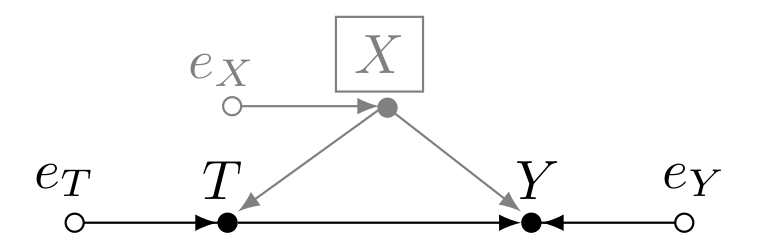
\includegraphics[width=0.65\linewidth,height=\textheight,keepaspectratio]{images/png/mdag_example1a.png}

}

\subcaption{\label{fig-mdag_example2}Conditioned DAG}

\end{minipage}%

\caption{\label{fig-example2}Plausible causal structure the scenario
outlined in Section~\ref{sec-appendixB2}.}

\end{figure}%

\paragraph{From probability to causality}\label{sec-appendixB33}

The structural approach to causal inference translates probabilistic
insights into actionable strategies seeking to identify the ACE from
associational quantities. The approach achieves this by relying on the
\emph{modularity assumption}, which posits that intervening on a node
alters only the causal mechanism of that node, leaving others unchanged
\citep[pp.~34]{Neal_2020}.

The modularity assumption underpins the concepts of manipulated graphs
and Truncated Factorization, which are essential for representing
interventions \(P(Y_{i} \:|\:do(T_{i}=t))\) within SCMs and DAGs.
\emph{Manipulated graphs} simulate physical interventions by removing
specific edges from a DAG, while preserving the remaining structure
unchanged \citep[pp.~34]{Neal_2020}. In parallel, \emph{Truncated
Factorization} (TF) achieves a similar simulation by removing specific
functions from the conceptual model and replacing them with constants,
while keeping the rest of the structure unchanged \citep{Pearl_2010}.
The probabilistic implications of this factorization are formalized in
Equation~\ref{eq-trunc_factor}, where \(S\) represents the subset of
variables \(X_{p}\) directly influenced by the intervention, while an
example illustrating these concepts follows below.

\begin{equation}\phantomsection\label{eq-trunc_factor}{
P(X_{1}, X_{2}, \dots, X_{P} \:|\:do(S)) =
\begin{cases}
  \prod P(X_{p} \:|\:pa(X_{p}) ) & \text{if} \: p \not\in S \\
  1 \quad & \text{otherwise}
\end{cases}
}\end{equation}

Using the TF, researchers can define the \emph{backdoor adjustment} to
identify the ACE. This adjustment states that if a variable
\(X_{p} \in S\) serves as a \emph{sufficient adjustment set} for the
effect of \(X_{a}\) on \(X_{b}\), then the ACE can be identified using
Equation~\ref{eq-backdoor}. The sufficient adjustment set (potentially
empty) must block all non-causal paths between \(X_{a}\) and \(X_{b}\)
without introducing new paths. If such a set exists, then \(X_{a}\) and
\(X_{b}\) are \emph{d-separated} by \(X_{p}\)
(\(X_{a} \:\bot\:X_{b} \:|\:X_{p}\)) \citep{Pearl_2009}, and \(X_{p}\)
satisfies the \emph{backdoor criterion} \citep[pp.~37]{Neal_2020}.

\begin{equation}\phantomsection\label{eq-backdoor}{
P(X_{a} \:|\:do(X_{b}=x)) = \sum_{Xp} P(X_{a} \:|\:X_{b}=x, X_{p}) P(X_{p})
}\end{equation}

Ultimately, the backdoor adjustment enables researchers to express the
ACE as:

\begin{equation}\phantomsection\label{eq-backdoor_adjustment}{
\begin{aligned}
\tau & = E[X_{a} \:|\:do(X_{b}=1)]- E[X_{a} \:|\:do(X_{b}=2)] \\
  & = E_{Xp}\left[ E[X_{a} \:|\:do(X_{b}=1), X_{p}]- E[X_{a} \:|\:do(X_{b}=2), X_{p}] \right] \\
  & = \sum_{Xp} X_{a} \cdot P(X_{a} \:|\:X_{b}=1, X_{p}) \cdot P(X_{p}) - \sum_{Xp} X_{a} \cdot P(X_{a} \:|\:X_{b}=2, X_{p}) \cdot P(X_{p})
\end{aligned}
}\end{equation}

With these new insights, researchers revisiting the scenario in
Section~\ref{sec-appendixB32} can infer that the socio-economic status
of the school, \(X\), satisfies the backdoor criterion, assuming the
causal structure depicted by the SCM \ref{fig-scm_example2} and DAG
\ref{fig-mdag_example2} is correct. This means that \(X\) serves as a
sufficient adjustment set, as it effectively blocks all confounding
non-causal paths introduced by the fork structure. Nevertheless, since
\(Y\) remains dependent on \(T\) even after conditioning
\((Y \:\not\bot\:T \:|\:X)\), this dependency can only be attributed to
the direct causal effect \(T \rightarrow Y\). Notably, for the purpose
of identification, the conditioned DAG \ref{fig-mdag_example2} is
equivalent to the manipulated DAG \ref{fig-mdag_example3}, because \(X\)
satisfies the backdoor criterion.

\begin{figure}

\begin{minipage}{0.50\linewidth}

\centering{

\[
\begin{aligned}
  X & := f_{X}(e_{X}) \\
  T & := t \\
  Y & := f_{Y}(t,X,e_{Y}) \\
  e_{T} & \:\bot\:e_{X} \\
  e_{T} & \:\bot\:e_{Y} \\
  e_{X} & \:\bot\:e_{Y}
\end{aligned}
\]

}

\subcaption{\label{fig-scm_example3}SCM}

\end{minipage}%
%
\begin{minipage}{0.50\linewidth}

\centering{

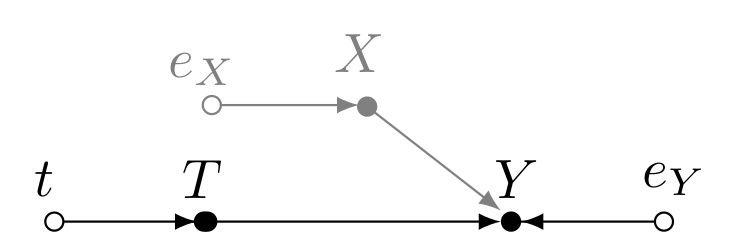
\includegraphics[width=0.65\linewidth,height=\textheight,keepaspectratio]{images/png/mdag_example1b.png}

}

\subcaption{\label{fig-mdag_example3}Manipulated DAG}

\end{minipage}%

\caption{\label{fig-example3}Plausible causal structure the scenario
outlined in Section~\ref{sec-appendixB32}.}

\end{figure}%

Researchers can then apply the \emph{backdoor adjustment} to identify
the ACE of \(T\) on \(Y\). They achieve this by first identifying the
CACE of \(T\) on \(Y\) by conditioning on \(X\), and then marginalizing
this effect over \(X\) to obtain the ACE. This process is expressed in
Equation~\ref{eq-mACE2} (see Section~\ref{sec-appendixB2}).

\begin{equation}\phantomsection\label{eq-mACE2}{
\begin{aligned}
  \tau & = E[Y_{i} \:|\:do(T_{i}=1)]- E[Y_{i} \:|\:do(T_{i}=2)] \\
  & = E_{X}\left[ E[Y_{i} \:|\:T_{i}=1, X] - E[Y_{i} \:|\:T_{i}=2, X] \right] \\
  & = \sum_{X} Y_{i} \cdot P( Y_{i} \:|\:T_{i}=1, X) \cdot P(X) - \sum_{X} Y_{i} \cdot P( Y_{i} \:|\:T_{i}=2, X) \cdot P(X)
\end{aligned}
}\end{equation}

\paragraph{The estimation process}\label{sec-appendixB34}

Ultimately, researchers can use Bayesian inference methods to estimate
the ACE. The approach begins by defining two probability distributions:
the likelihood of the data,
\(P(X_{1}, X_{2}, \dots, X_{P} \:|\:\theta)\), and the prior
distribution, \(P(\theta)\) \citep{Everitt_et_al_2010}, where \(X_{P}\)
represents a random variable, and \(\theta\) represents a
one-dimensional parameter space for simplicity. After observing
empirical data, researchers can update the priors to posterior
distributions using Bayes' rule in Equation~\ref{eq-bayes_rule}:

\begin{equation}\phantomsection\label{eq-bayes_rule}{
P(\theta \:|\:X_{1}, X_{2}, \dots, X_{P}) = \frac{P(X_{1}, X_{2}, \dots, X_{P} \:|\:\theta) \cdot P(\theta)}{P(X_{1}, X_{2}, \dots, X_{P})}
}\end{equation}

Given that the denominator on the right-hand side of
Equation~\ref{eq-bayes_rule} serves as a normalizing constant
independent of the parameter \(\theta\), researchers can simplify the
posterior updating process into three steps. First, they integrate new
empirical data through the likelihood. Second, they update the
parameters' priors to a posterior distribution according to
Equation~\ref{eq-prop_rule}. Ultimately, they normalize these results to
obtain a valid probability distribution.

\begin{equation}\phantomsection\label{eq-prop_rule}{
P(\theta \:|\:X_{1}, X_{2}, \dots, X_{P}) \propto P(X_{1}, X_{2}, \dots, X_{P}\:|\:\theta) \cdot P(\theta)
}\end{equation}

Temporarily setting aside the definition of prior distributions
\(P(\theta)\), note that the posterior updating process depends heavily
on the assumptions underlying the likelihood of the data. However, as
the number of random variables, \(P\), increases, this joint
distribution quickly becomes intractable \citep{Neal_2020}. This
intractability is evident from Equation~\ref{eq-like_chain}, where the
likelihood distribution is expressed by multiple chained CPDs.

\begin{equation}\phantomsection\label{eq-like_chain}{
P(X_{1}, X_{2}, \dots, X_{P} \:|\:\theta) = P(X_{1} \:|\:\theta) \prod^{P}_{p=2} P(X_{i} \:|\:X_{i-1}, \dots, X_{1}, \theta )
}\end{equation}

Nevertheless, researchers can manage the complexity of the likelihood by
assuming specific local (in)dependencies among variables. SCMs and DAGs
provide a formal framework to represent these assumptions, as detailed
in Section~\ref{sec-appendixB32}. These assumptions improve model
tractability and simplify the estimation process by enabling the
derivation of the BNF of the likelihood (Equation~\ref{eq-like_BNF}).
With this simplified structure, any probabilistic programming language
can model the system and compute the parameter's posterior distribution
using Equation~\ref{eq-bayes_rule}.

\begin{equation}\phantomsection\label{eq-like_BNF}{
P(X_{1}, X_{2}, \dots, X_{P} \:|\:\theta) = P(X_{1} \:|\:\theta) \prod^{P}_{p=2} P(X_{i} \:|\:pa(X_{i}), \theta )
}\end{equation}

\newpage{}

\section*{References}\label{references}
\addcontentsline{toc}{section}{References}

\renewcommand{\bibsection}{}
\bibliography{references.bib}





\end{document}
